\chapter{Manual de usuario}

\section{Introducción}

Nextinit es una plataforma de generación de ideas y fomento de la innovación. 

\section{Inicio de sesión}

Al abrir la aplicación aparece la pantalla para iniciar sesión (ver figura~\ref{fig:login}), es 
necesario ingresar el correo y la contraseña para entrar en la aplicación. Para posteriores 
veces no será necesario, a no ser, que se haya cerrado sesión en la aplicación.

\begin{figure}[!h]
	\begin{center}
		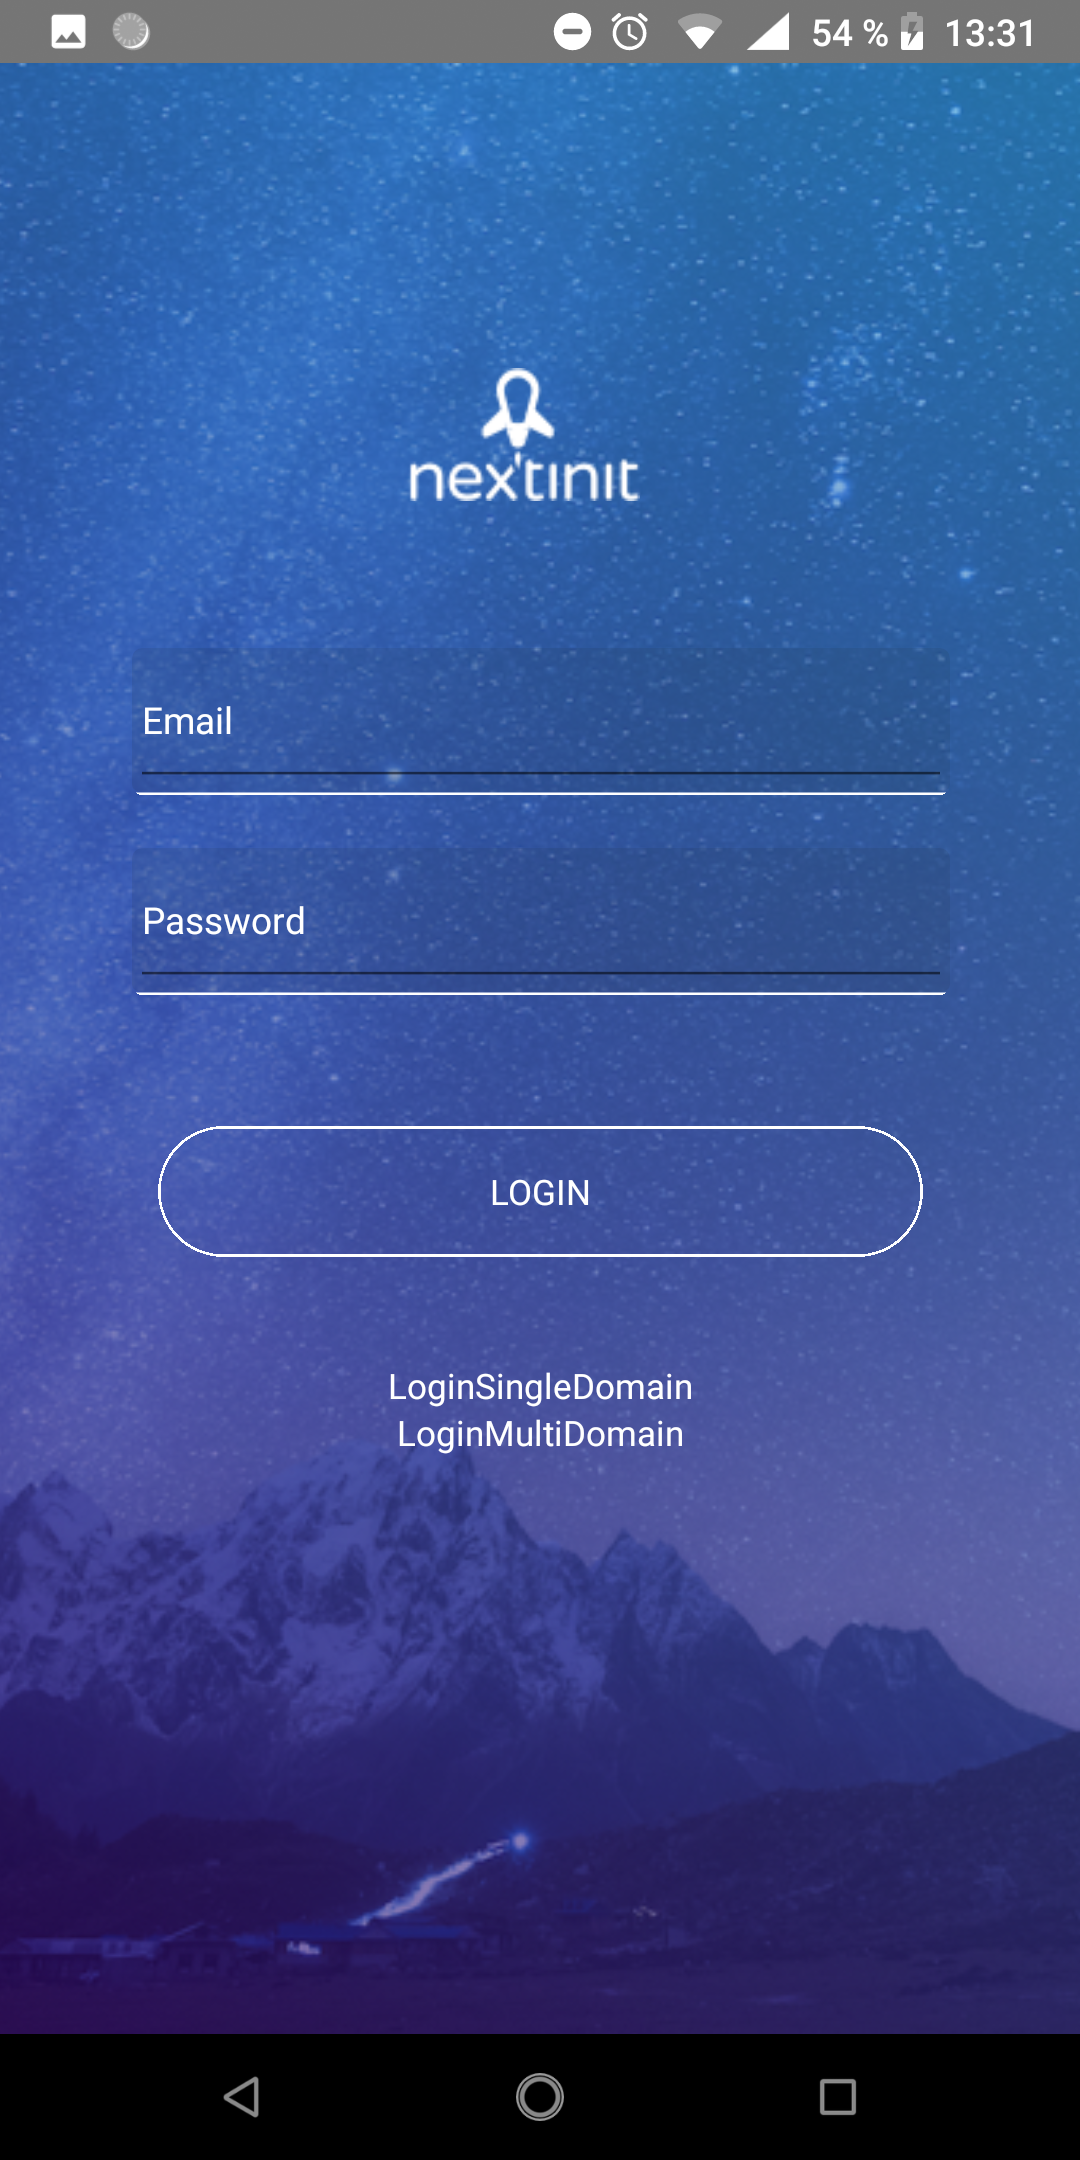
\includegraphics[width=0.3\textwidth]{./img/anexo1/login.png}
		\caption{Pantalla de inicio de sesión}
		\label{fig:login}
	\end{center}
\end{figure}

Una vez introducidos los datos correctos, en caso de disponer de más de un nextinit,
se mostrará la pantalla de selección de nextinit (ver figura~\ref{fig:seleccion_empresa}) 
donde se puede seleccionar el nextinit al que se quiere acceder.

\begin{figure}[!h]
	\begin{center}
		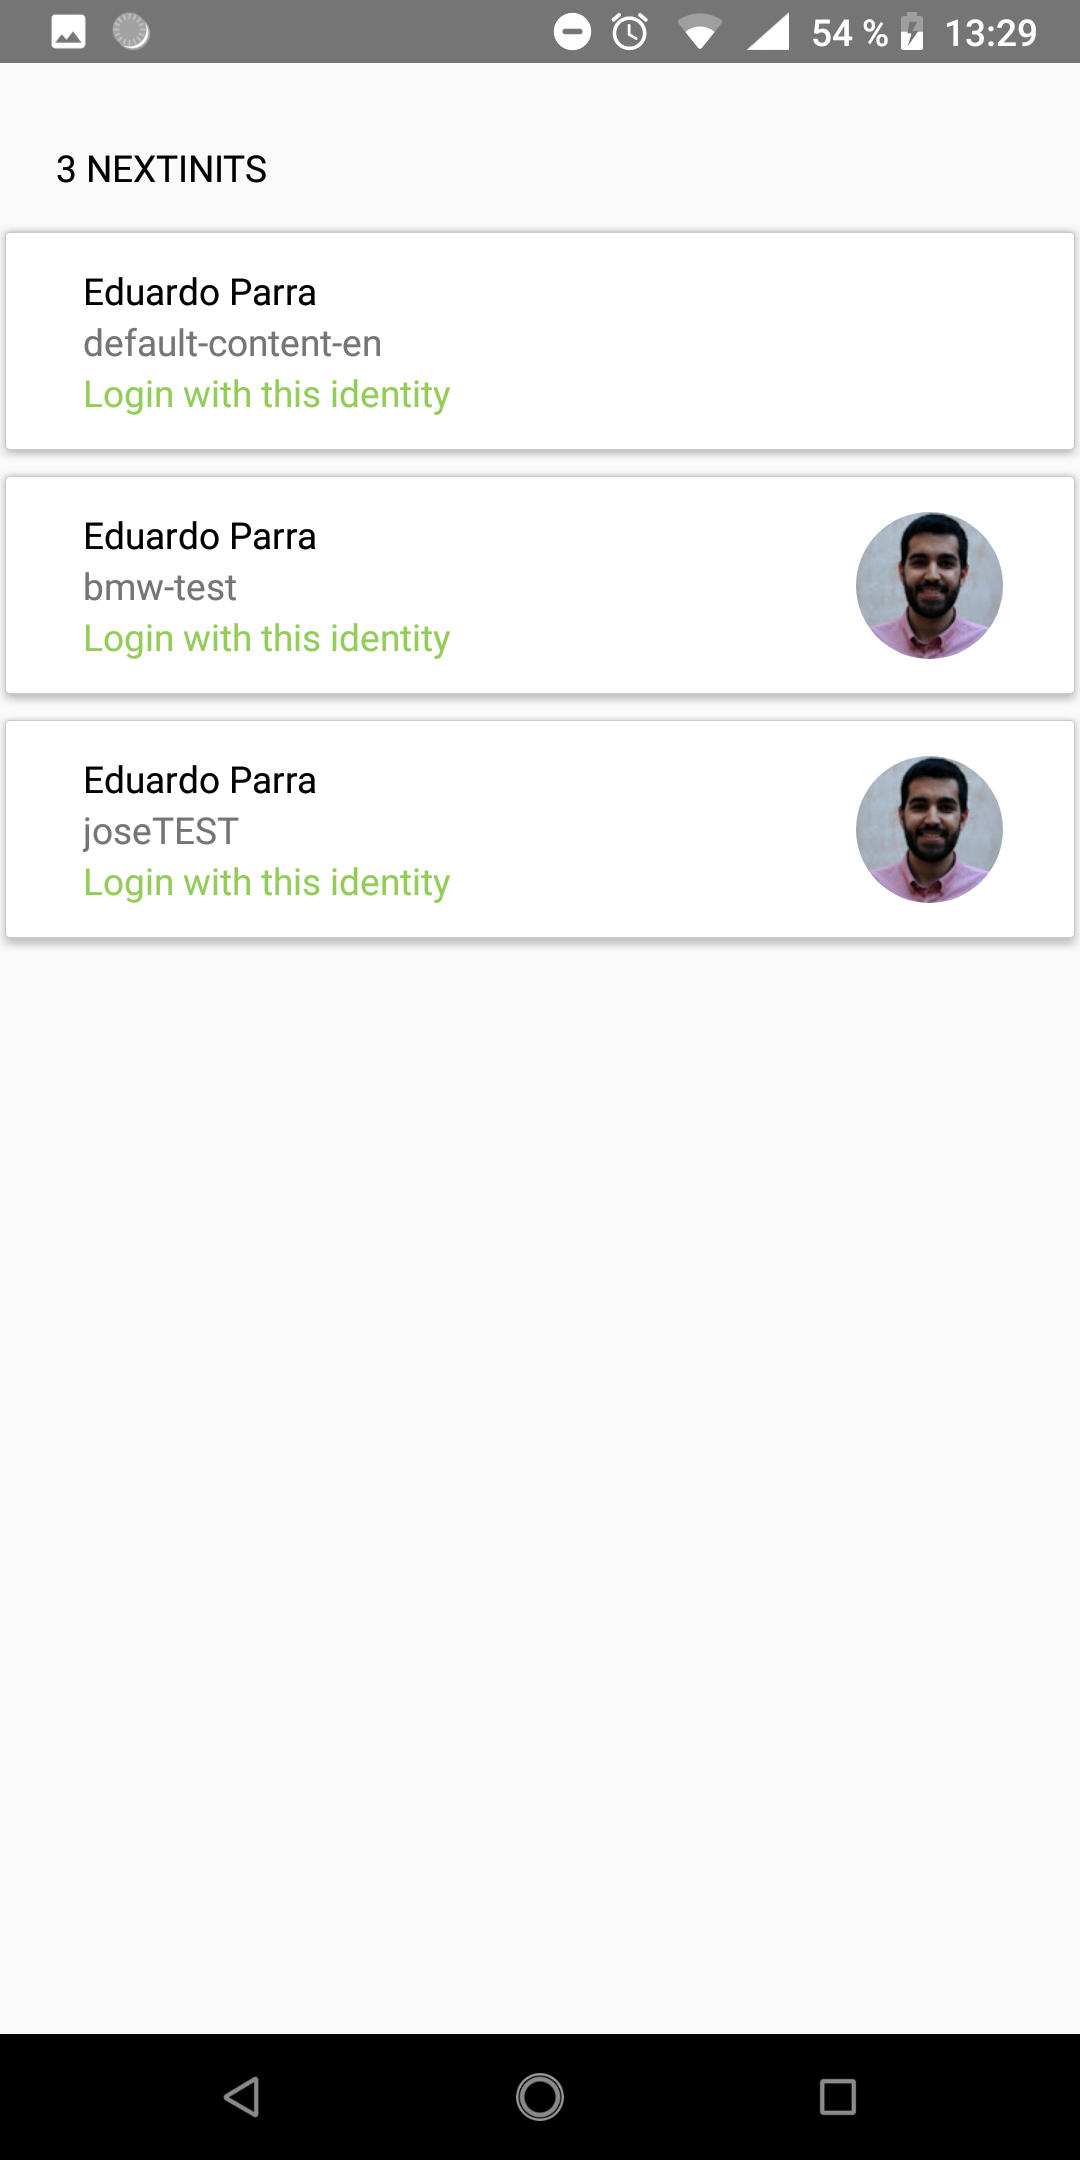
\includegraphics[width=0.3\textwidth]{./img/anexo1/seleccion_empresa.png}
		\caption{Pantalla de selección de Nextinit}
		\label{fig:seleccion_empresa}
	\end{center}
\end{figure}

\section{Inicio}
 
En la pantalla principal de Nextinit (ver figura~\ref{fig:inicio}) aparece un carrusel de desafíos 
(en caso de que el Nextinit lo tenga activados) desde el cual se puede acceder a la información 
del desafío. A continuación, se muestra una lista con todas las ideas del Nextinit, incluidas los 
borradores guardados del usuario.

\begin{figure}[!h]
	\begin{center}
		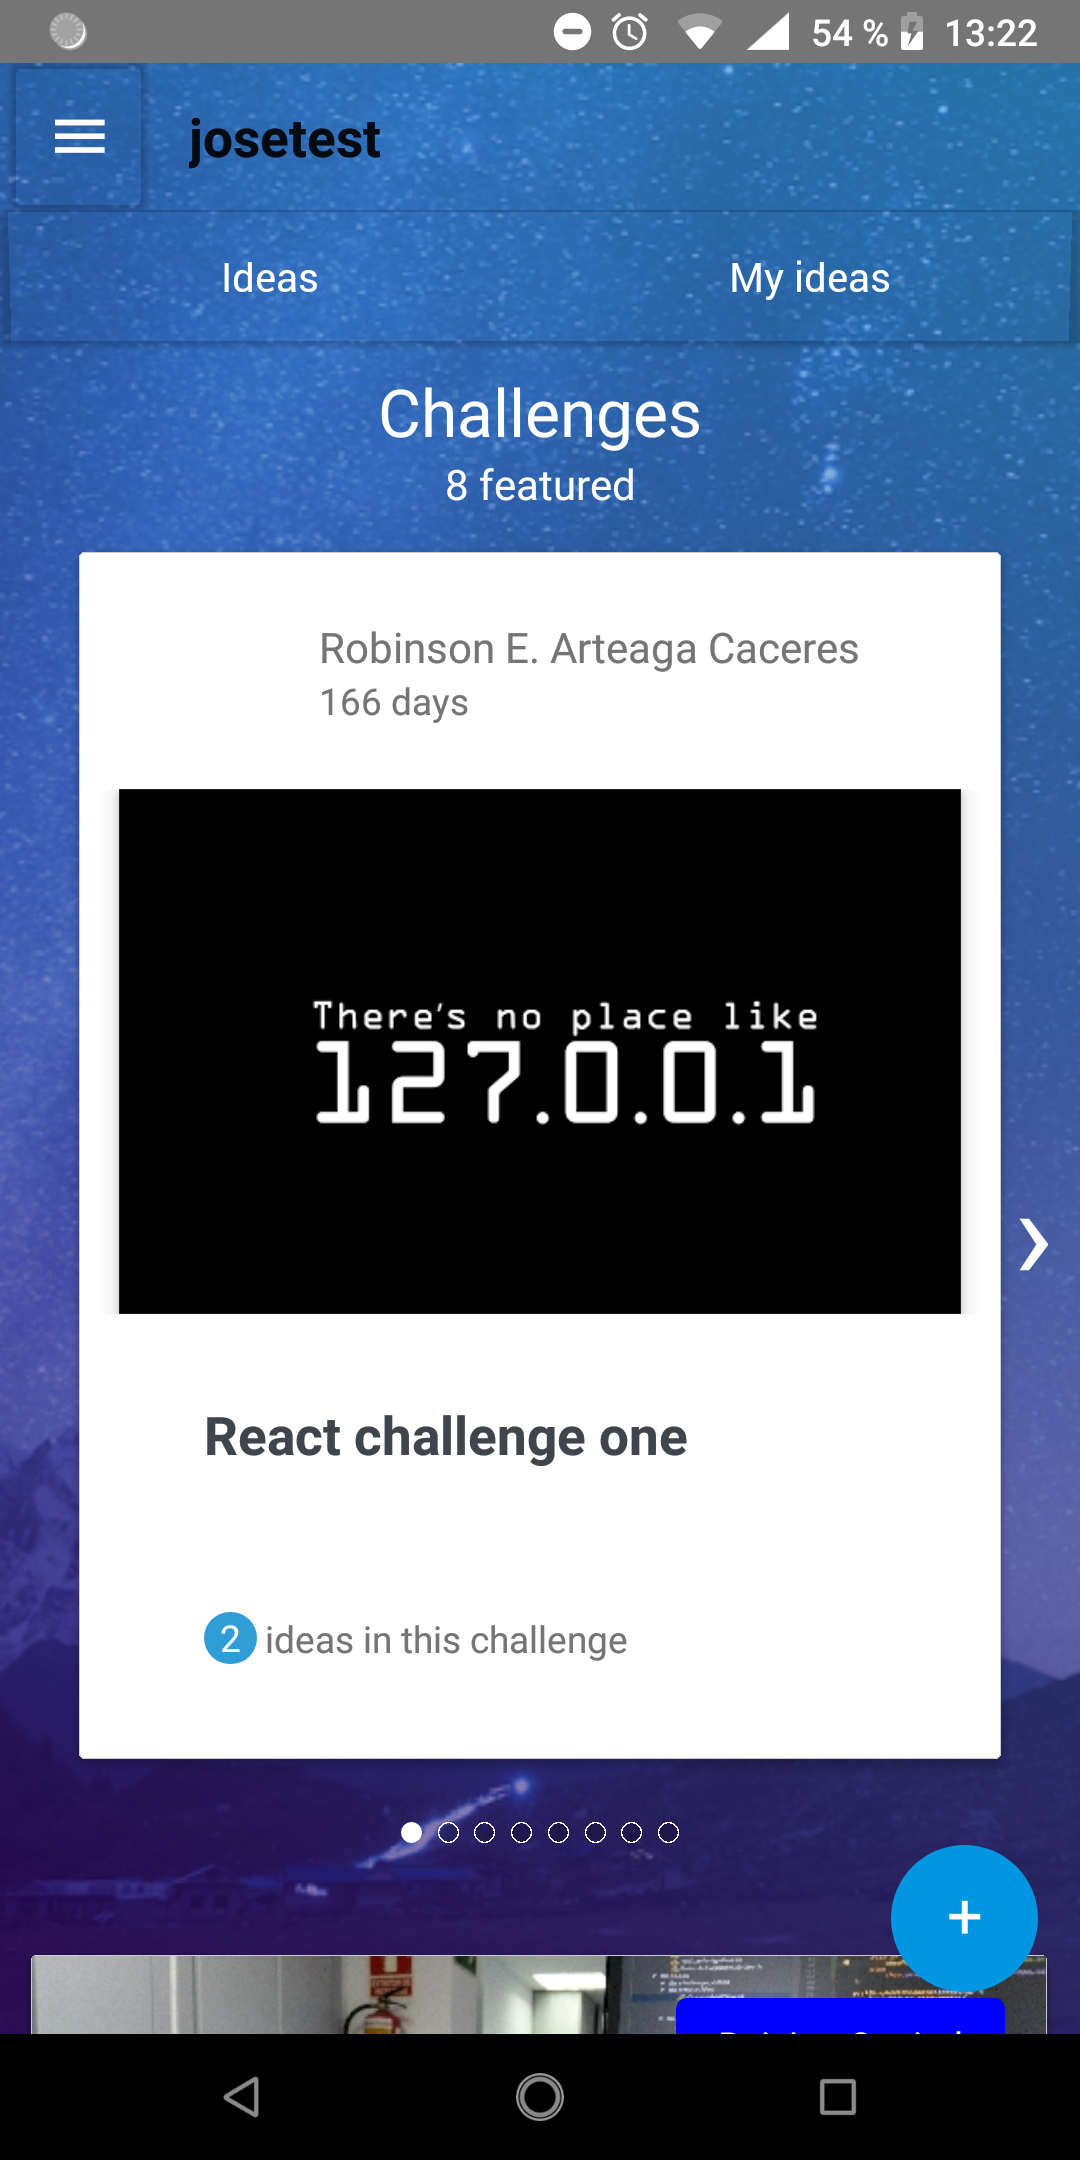
\includegraphics[width=0.3\textwidth]{./img/anexo1/inicio.png}
		\caption{Pantalla principal}
		\label{fig:inicio}
	\end{center}
\end{figure}

Para navegar por la aplicación existe un menú lateral (ver figura~\ref{fig:menu_admin}) al que 
se puede acceder deslizando desde la parte izquierda de la aplicación hacia la derecha o pulsando 
en el botón superior izquierdo de la pantalla.

\begin{figure}[!h]
	\begin{center}
		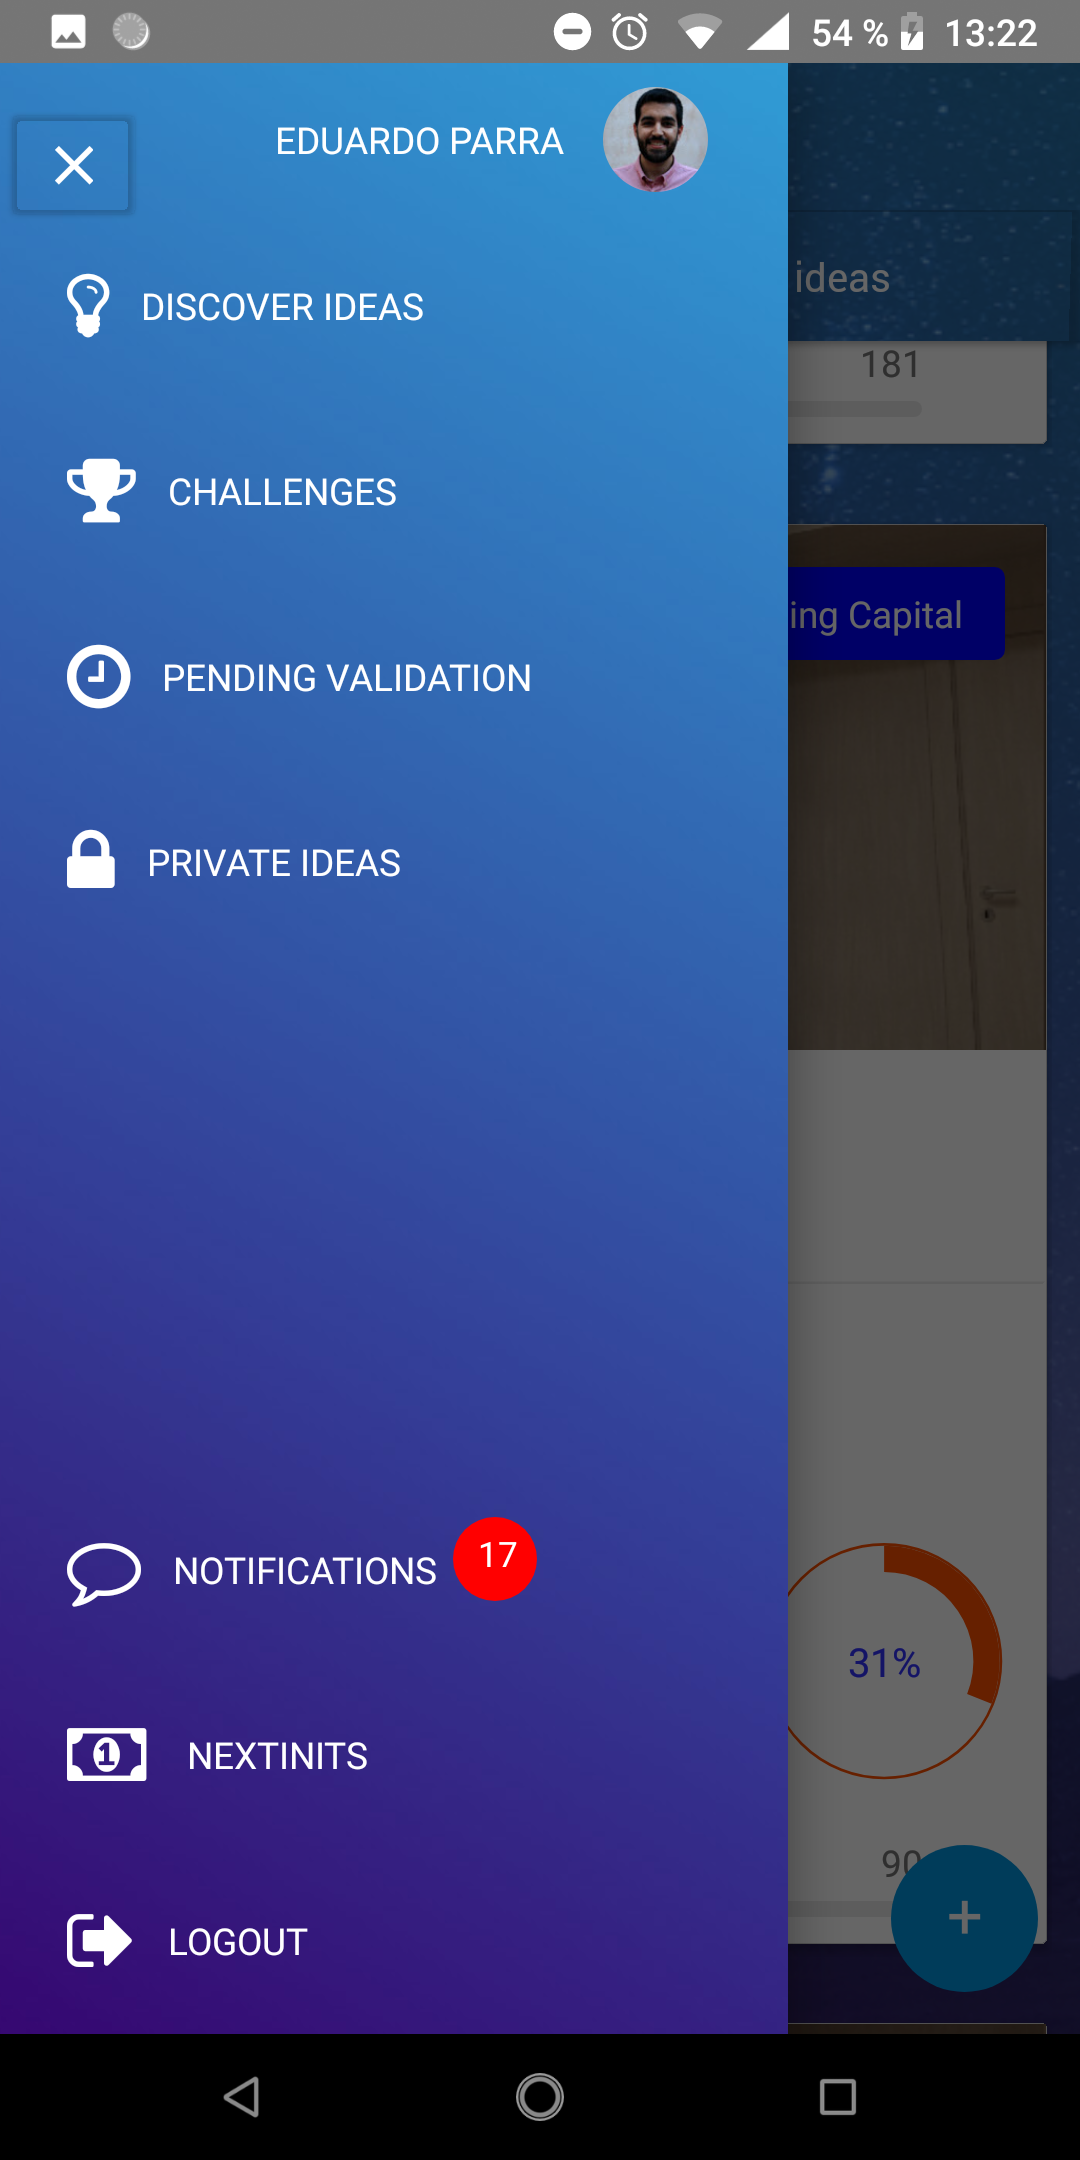
\includegraphics[width=0.3\textwidth]{./img/anexo1/menu_admin.png}
		\caption{Menú lateral de la aplicación}
		\label{fig:menu_admin}
	\end{center}
\end{figure}

\section{Ideas}

En la pestaña «Mis ideas» de la pantalla principal se muestra una lista con todas la ideas del usuario 
tanto las publicadas como las no publicadas (ver figura~\ref{fig:inicio_mis_ideas}).

\begin{figure}[!h]
	\begin{center}
		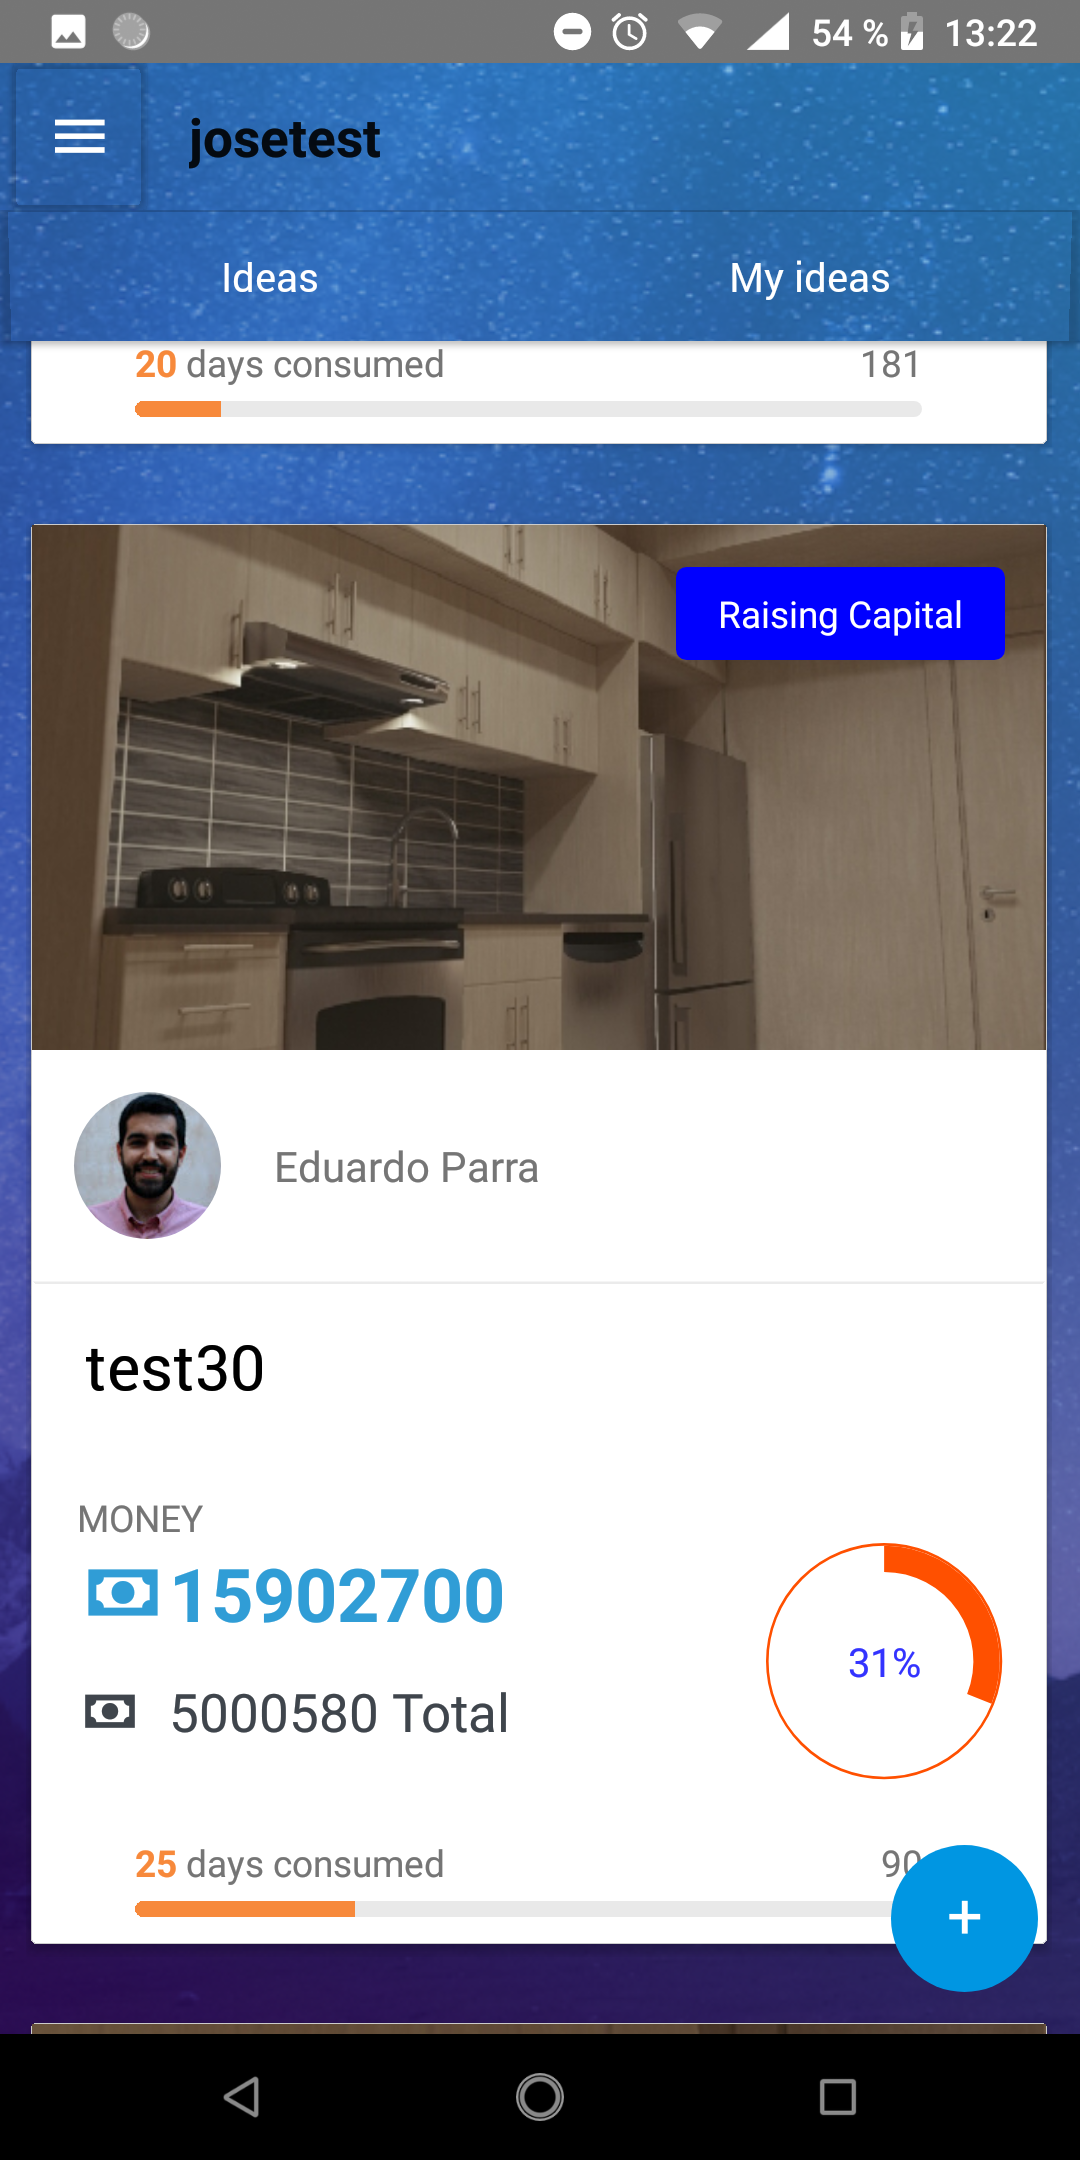
\includegraphics[width=0.3\textwidth]{./img/anexo1/inicio_mis_ideas.png}
		\caption{Pantalla de «Mis ideas»}
		\label{fig:inicio_mis_ideas}
	\end{center}
\end{figure}

Al pulsar en una idea de la lista se accede a la información de la idea. En la pantalla inicial 
de la idea se puede ver la descripción (ver figura~\ref{fig:ver_idea_inicio}), el desafío al que 
pertenece (en caso de pertenecer a alguno), El dinero recaudado y el restante, así como el porcentaje 
que incrementará los objetivos estratégicos de la organización.

\begin{figure}[!h]
	\begin{center}
		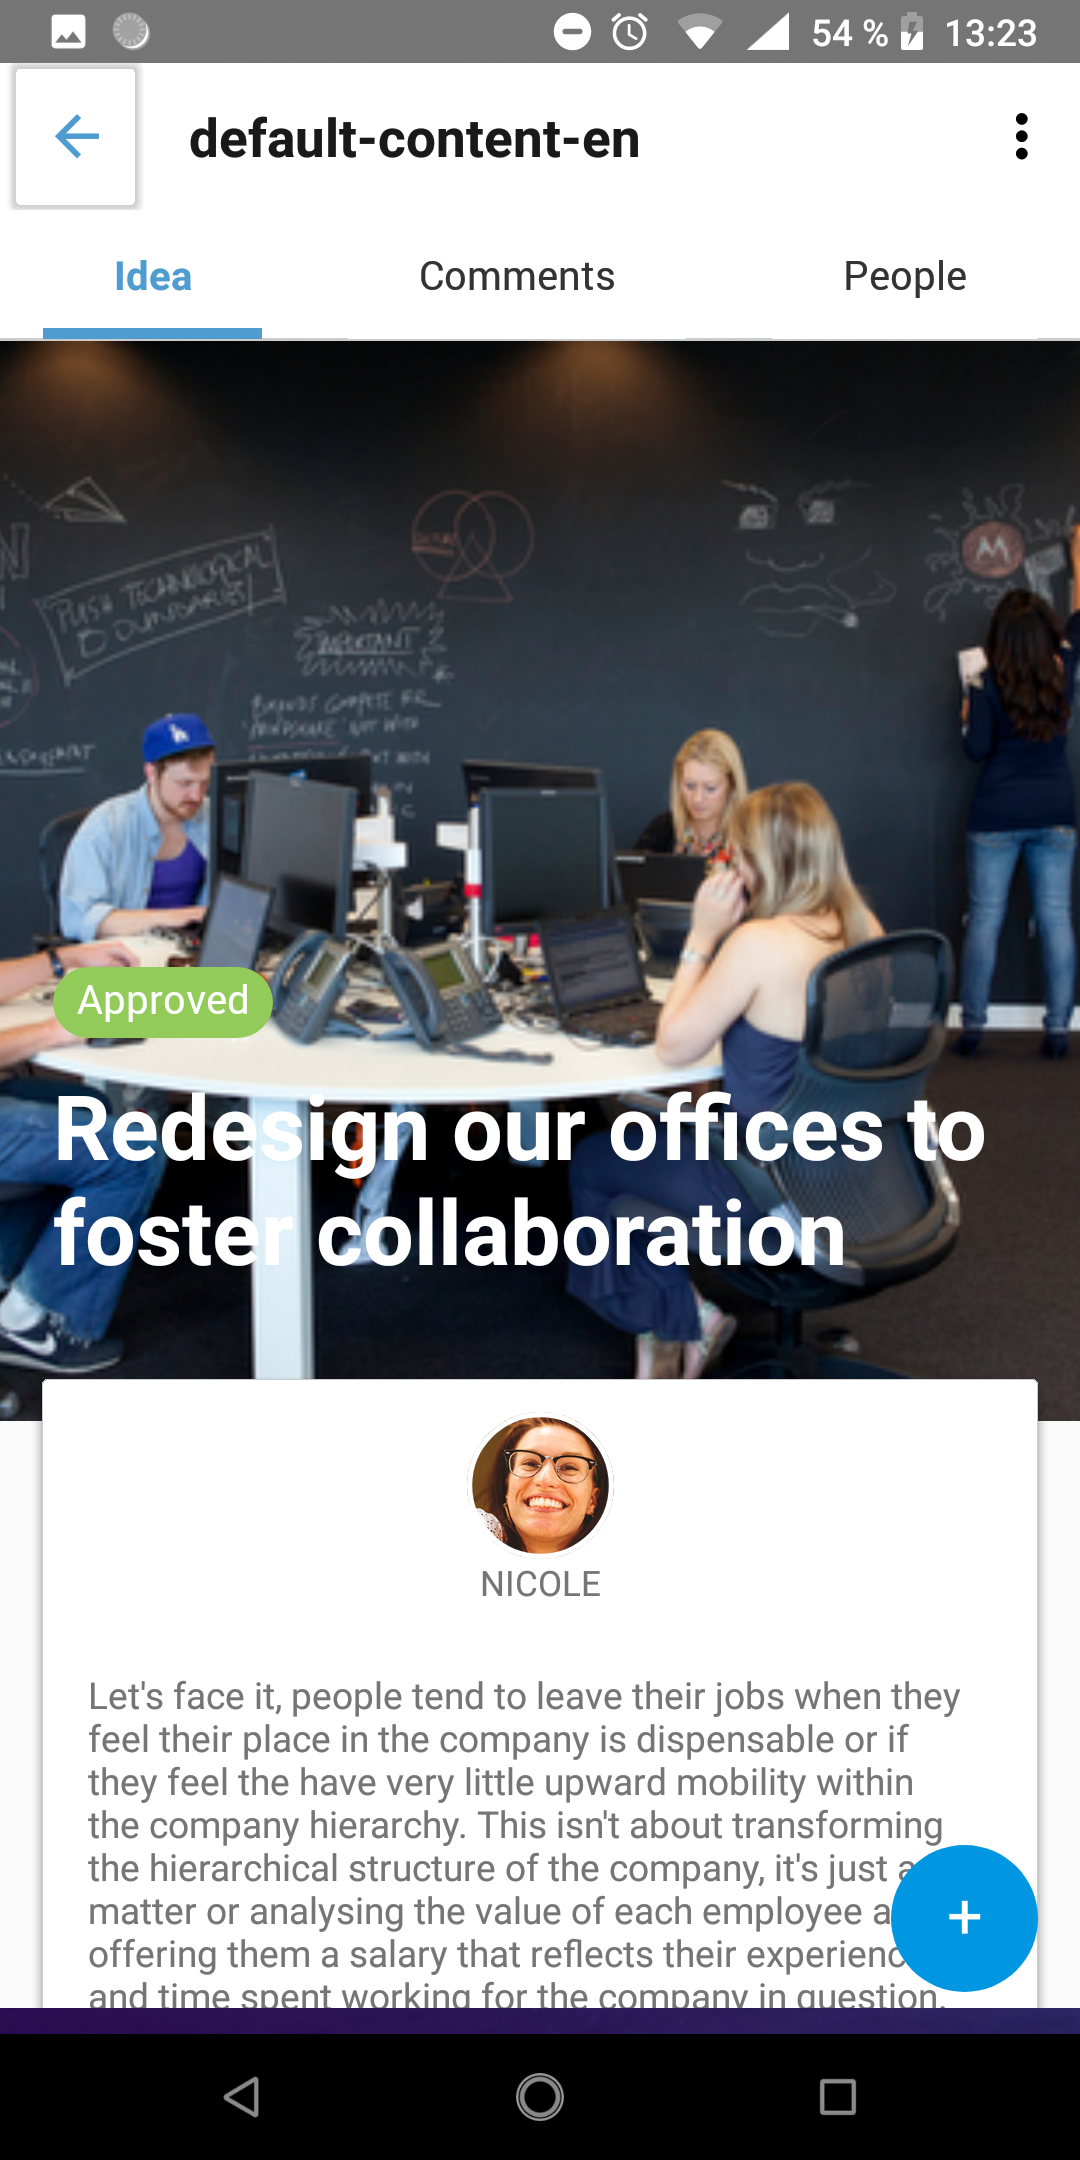
\includegraphics[width=0.3\textwidth]{./img/anexo1/ver_idea_inicio.png}
		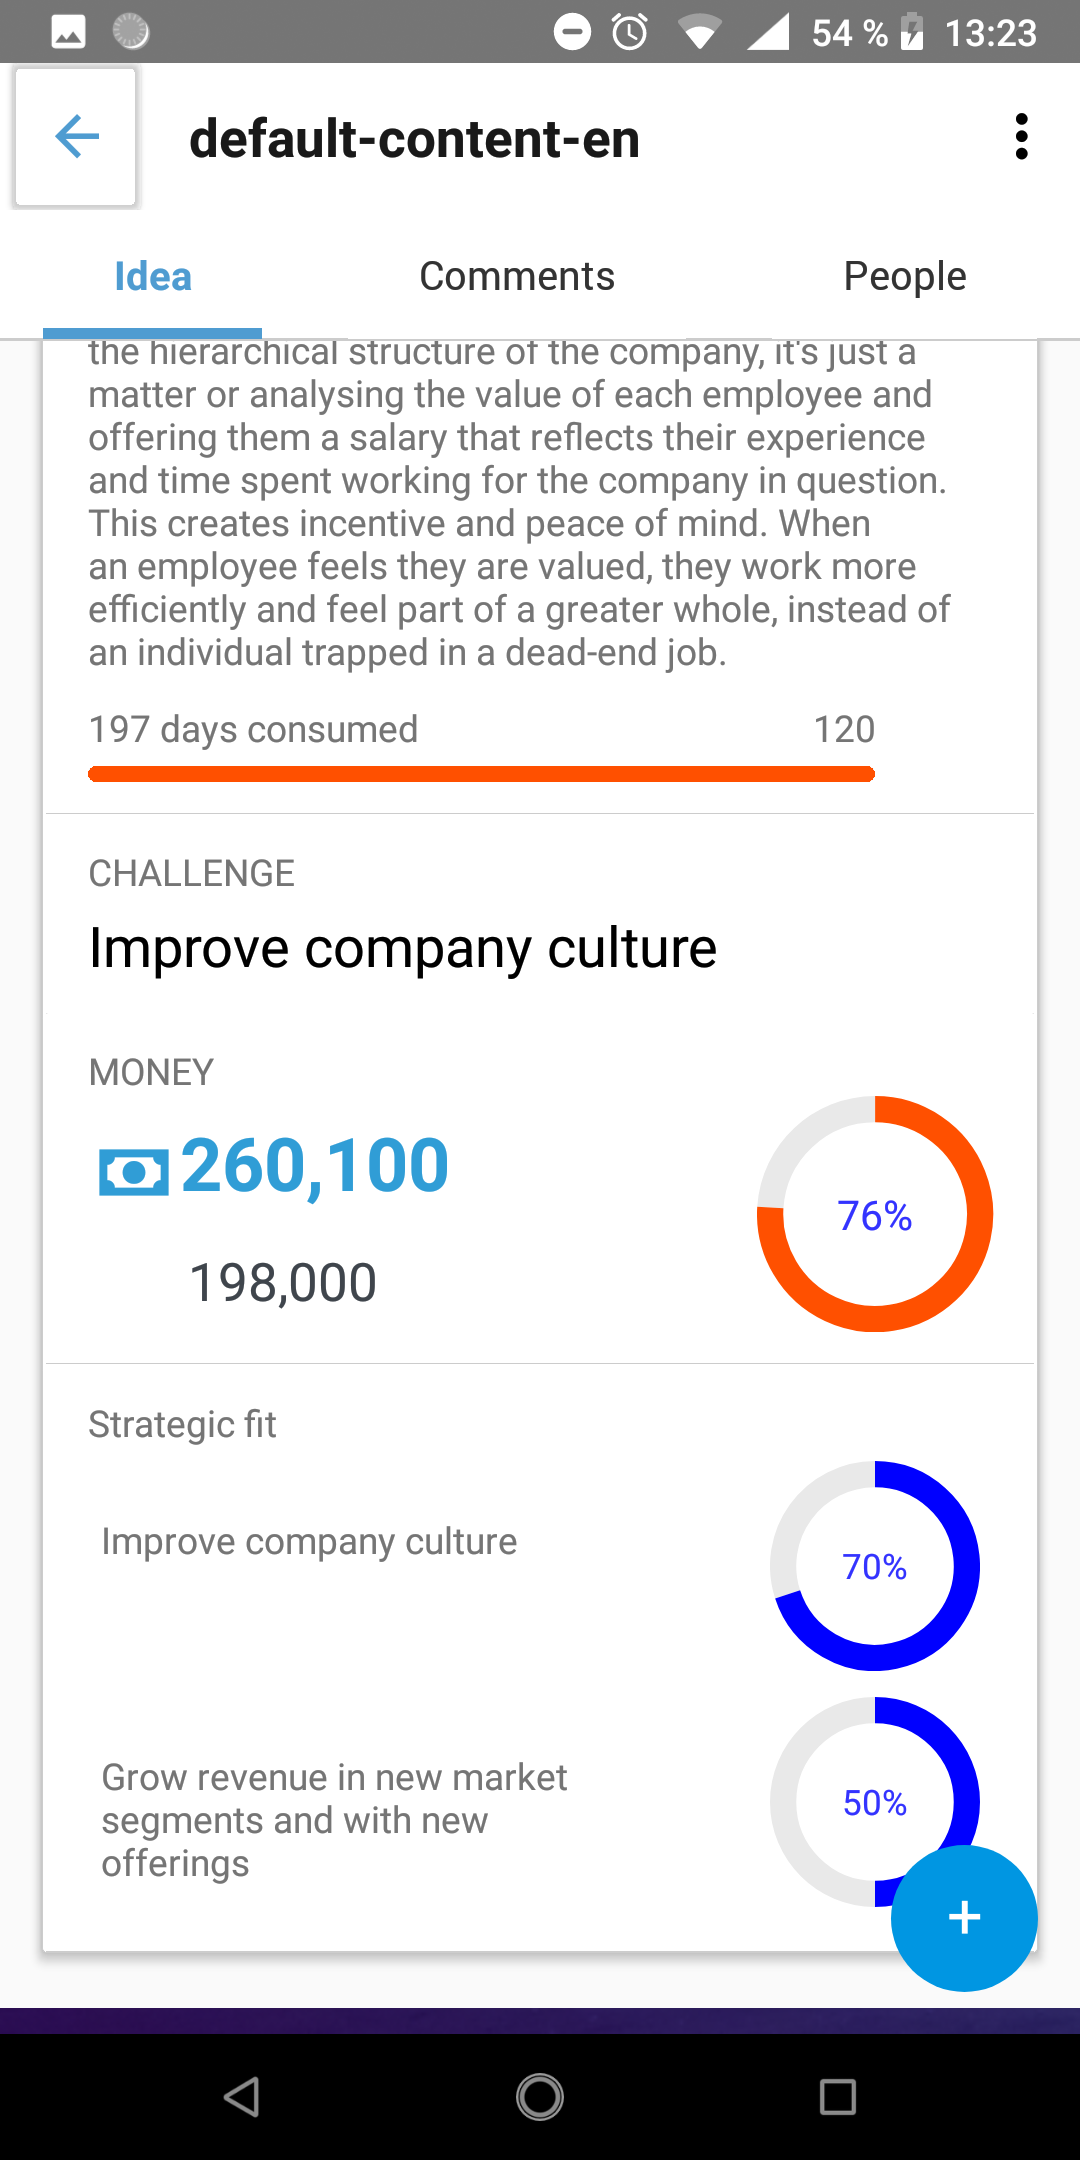
\includegraphics[width=0.3\textwidth]{./img/anexo1/ver_idea_inicio_cont.png}
		\caption{Pestaña inicial de la información de la idea}
		\label{fig:ver_idea_inicio}
	\end{center}
\end{figure}

En la pestaña de comentarios (ver figura~\ref{fig:ver_idea_comentarios}) se pueden ver los comentarios 
y las respuestas a estos que han dejado los usuarios de la organización. Además, los usuario pueden 
dar a «Me gusta» a los comentarios que deseen.

\begin{figure}[!h]
	\begin{center}
		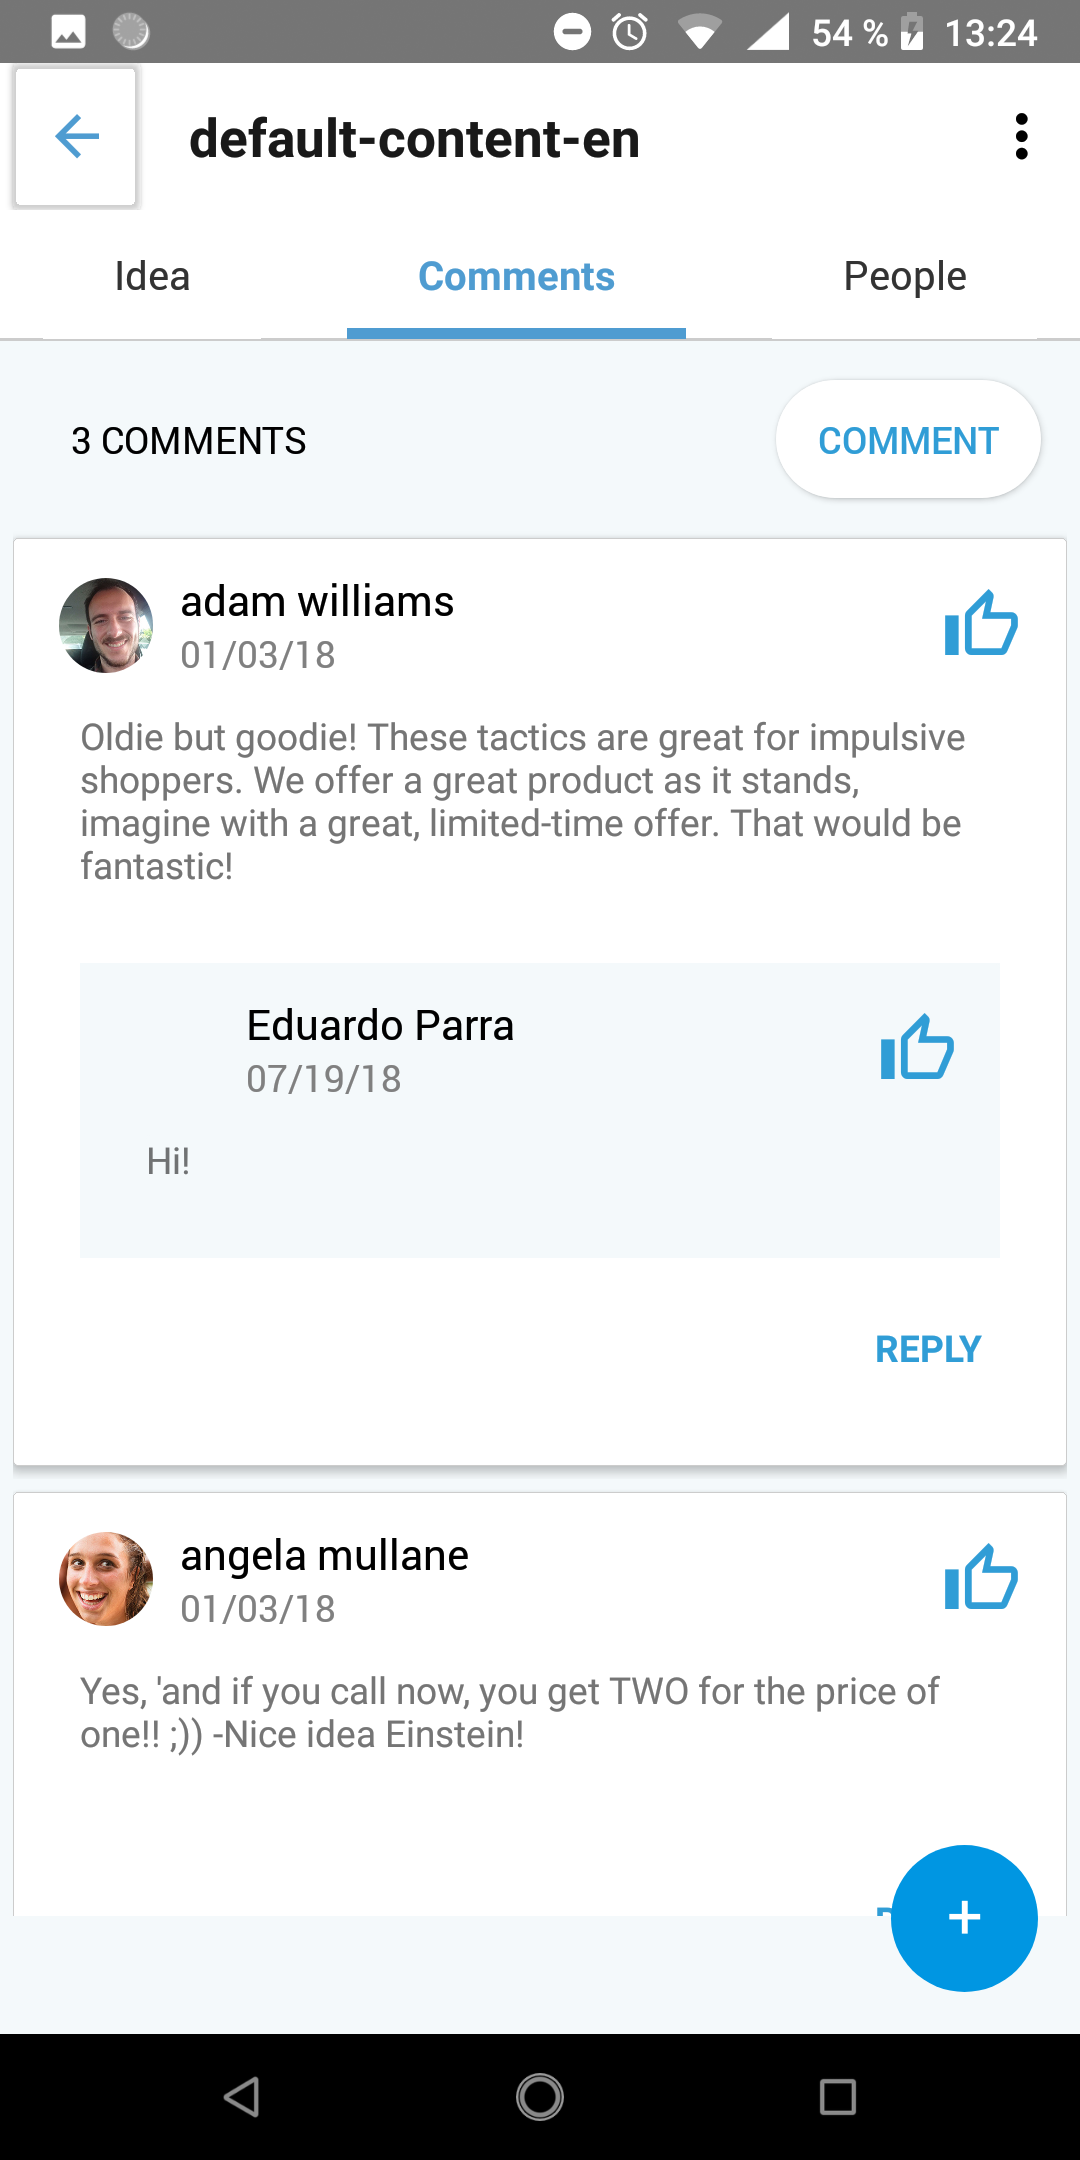
\includegraphics[width=0.3\textwidth]{./img/anexo1/ver_idea_comentarios.png}
		\caption{Pantalla de comentarios de la idea}
		\label{fig:ver_idea_comentarios}
	\end{center}
\end{figure}

En la pestaña «Gente» (ver figura~\ref{fig:ver_idea_gente}) se pueden ver las personas 
que han invertido en la idea, que forman el equipo de la idea, que colaboran con la idea o 
el equipo que ha propuesto la idea. En caso de que sean demasiados participantes para 
mostrarlos aparecerá unos pocos y para ver el resto habrá que pulsar el botón de al lado 
para mostrar las personas restantes.

\begin{figure}[!h]
	\begin{center}
		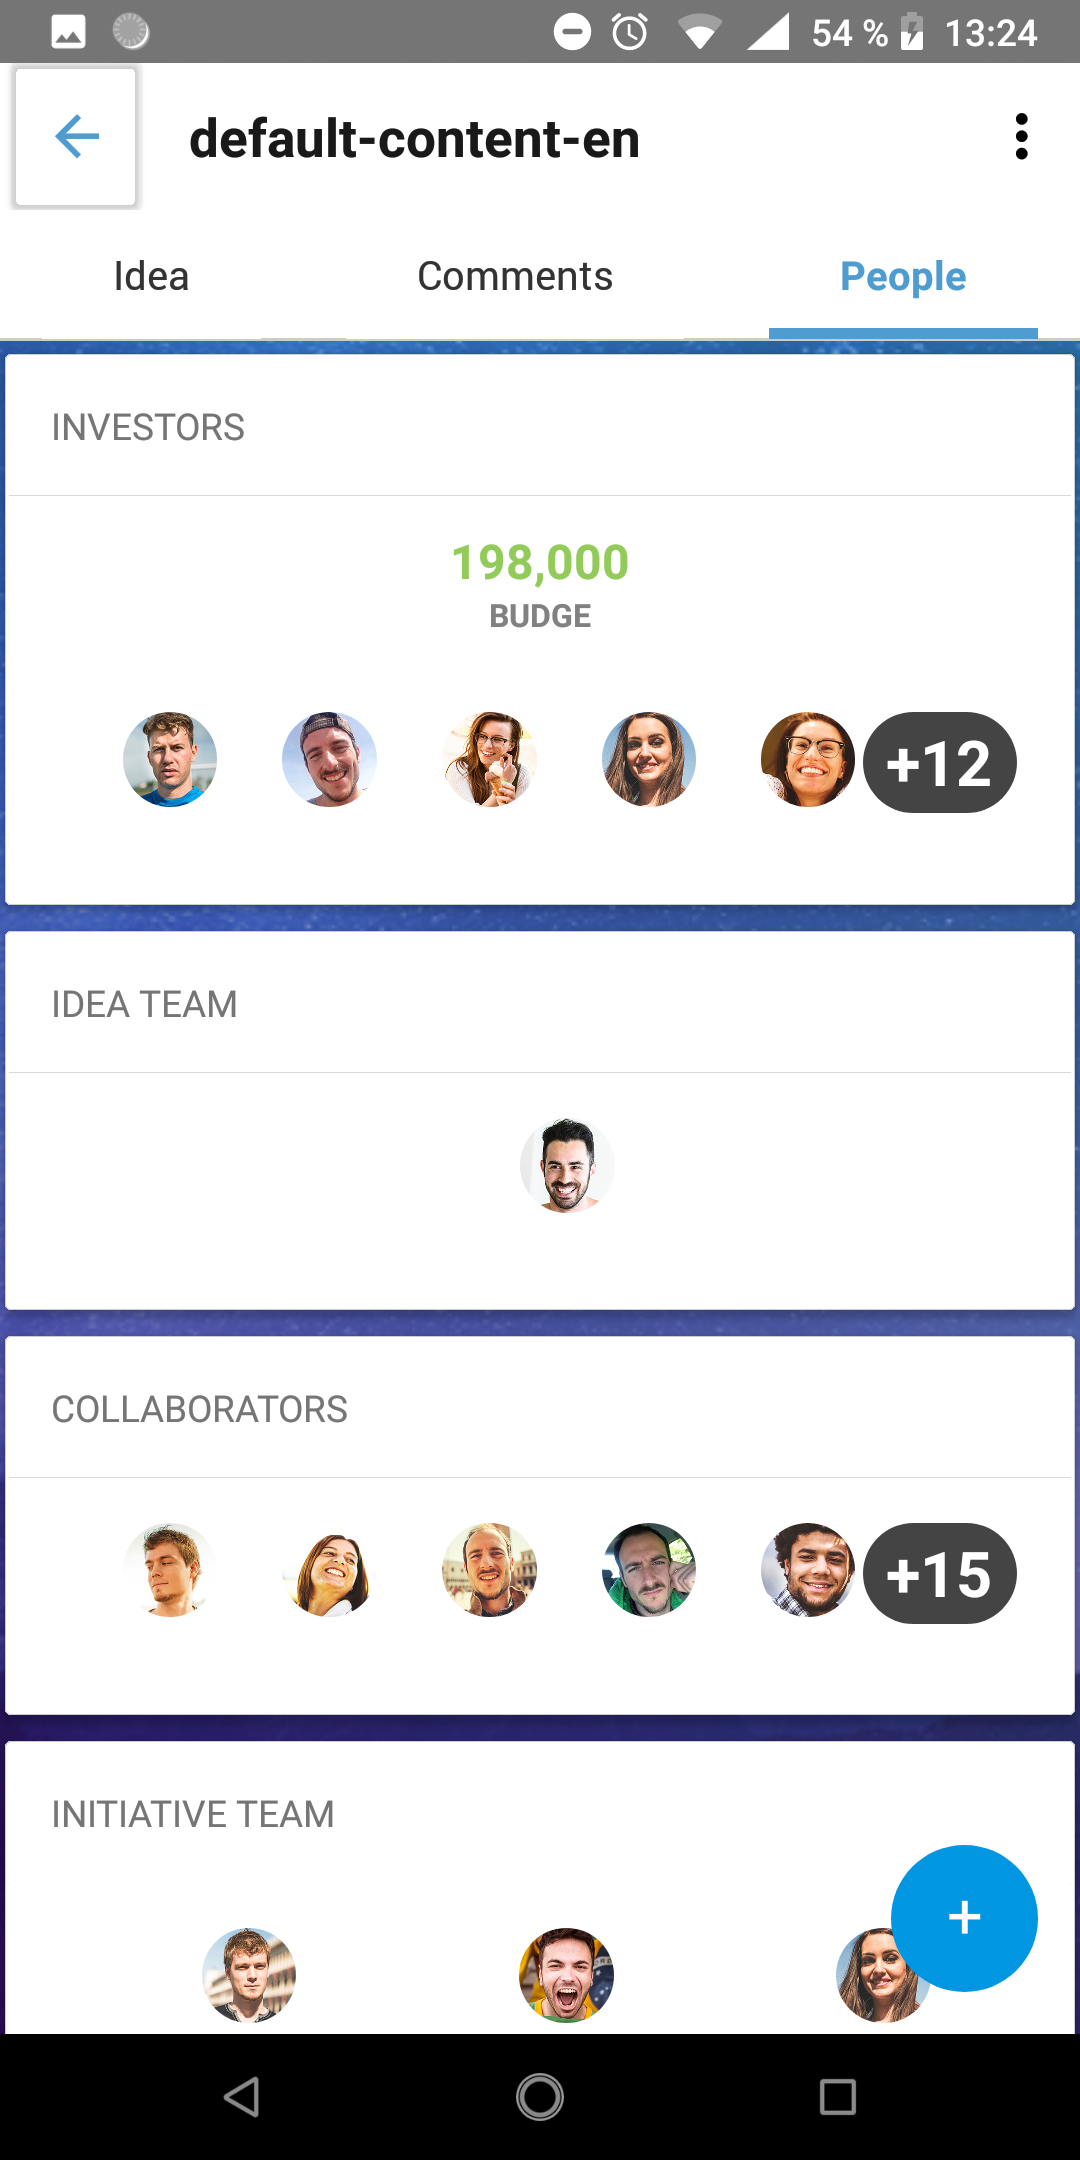
\includegraphics[width=0.3\textwidth]{./img/anexo1/ver_idea_gente.png}
		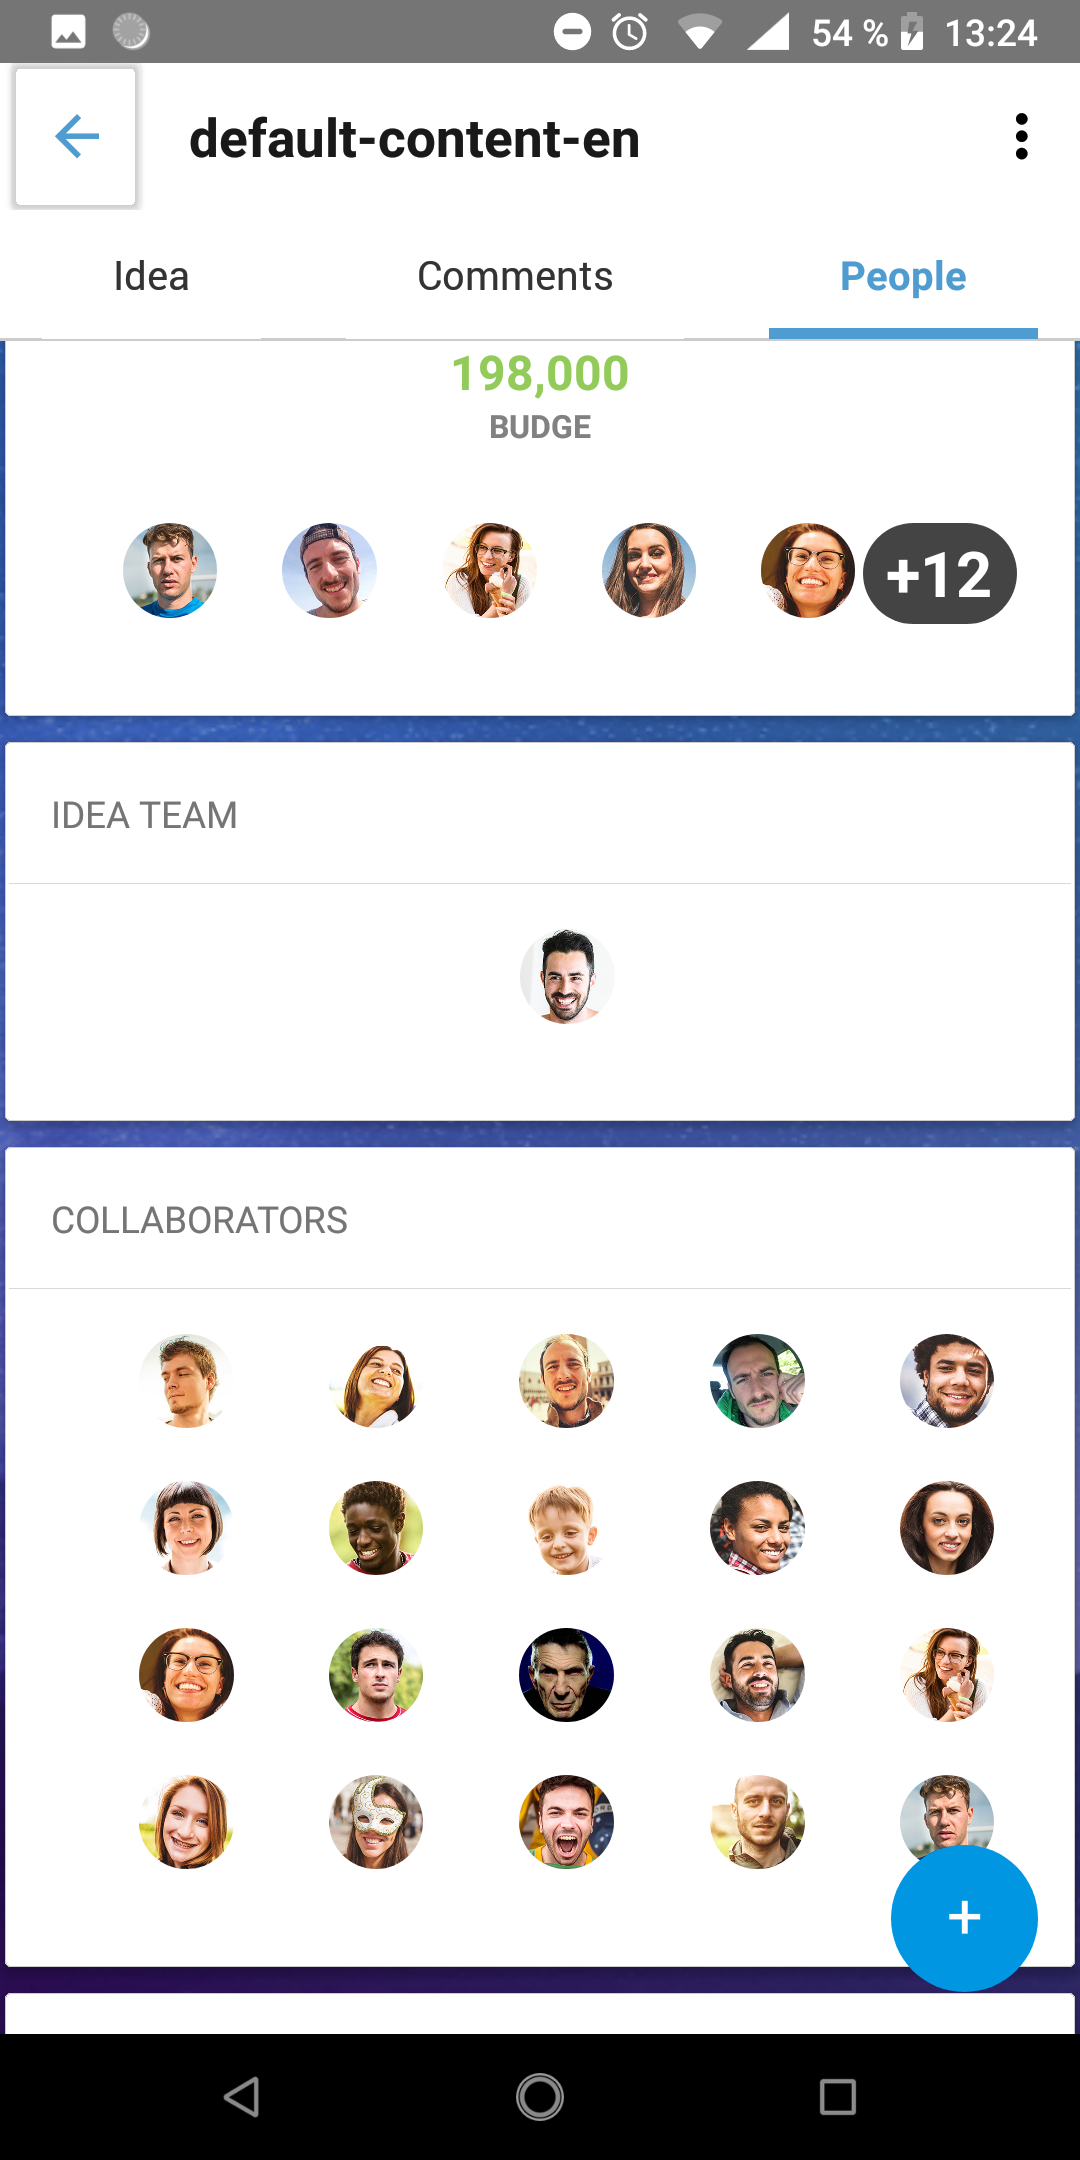
\includegraphics[width=0.3\textwidth]{./img/anexo1/ver_idea_gente_expandido.png}
		\caption{Pantalla de gente de la idea}
		\label{fig:ver_idea_gente}
	\end{center}
\end{figure}

\subsection{Crear una idea}

Se puede crear una idea desde la pantalla principal de la aplicación, pulsando en el botón 
«+» (ver figura~\ref{fig:inicio_crear_idea}), pueden ser ideas públicas, que las verán todos 
los usuarios del Nextinit o privadas, que solo las verán los administradores.

\begin{figure}[!h]
	\begin{center}
		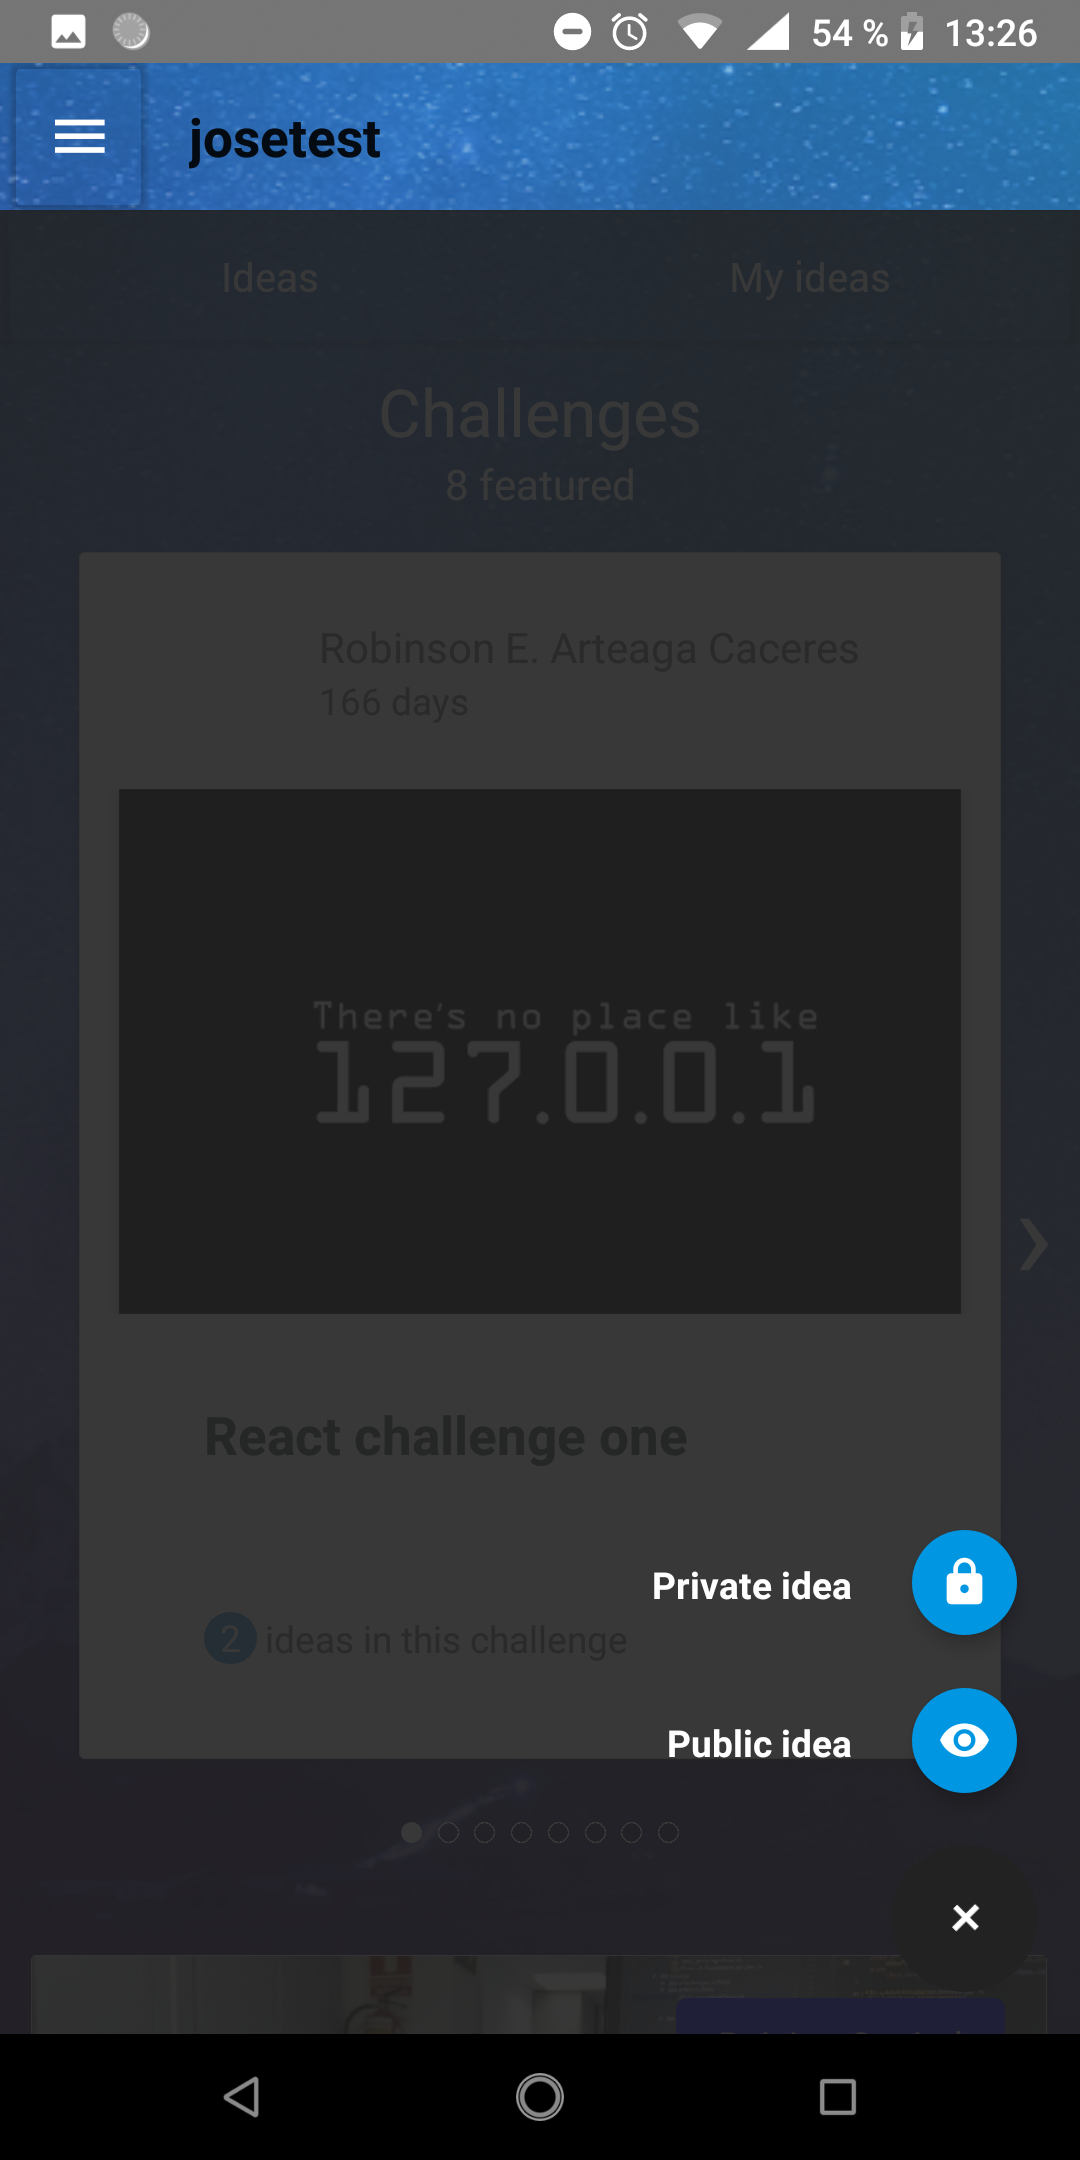
\includegraphics[width=0.3\textwidth]{./img/anexo1/inicio_crear_idea.png}
		\caption{Botón de crear idea}
		\label{fig:inicio_crear_idea}
	\end{center}
\end{figure}

Aparecerá un formulario para crear la idea (ver figura~\ref{fig:crear_idea}) en él, el usuario 
debe introducir al menos un título, una descripción y una imagen.

\begin{figure}[!h]
	\begin{center}
		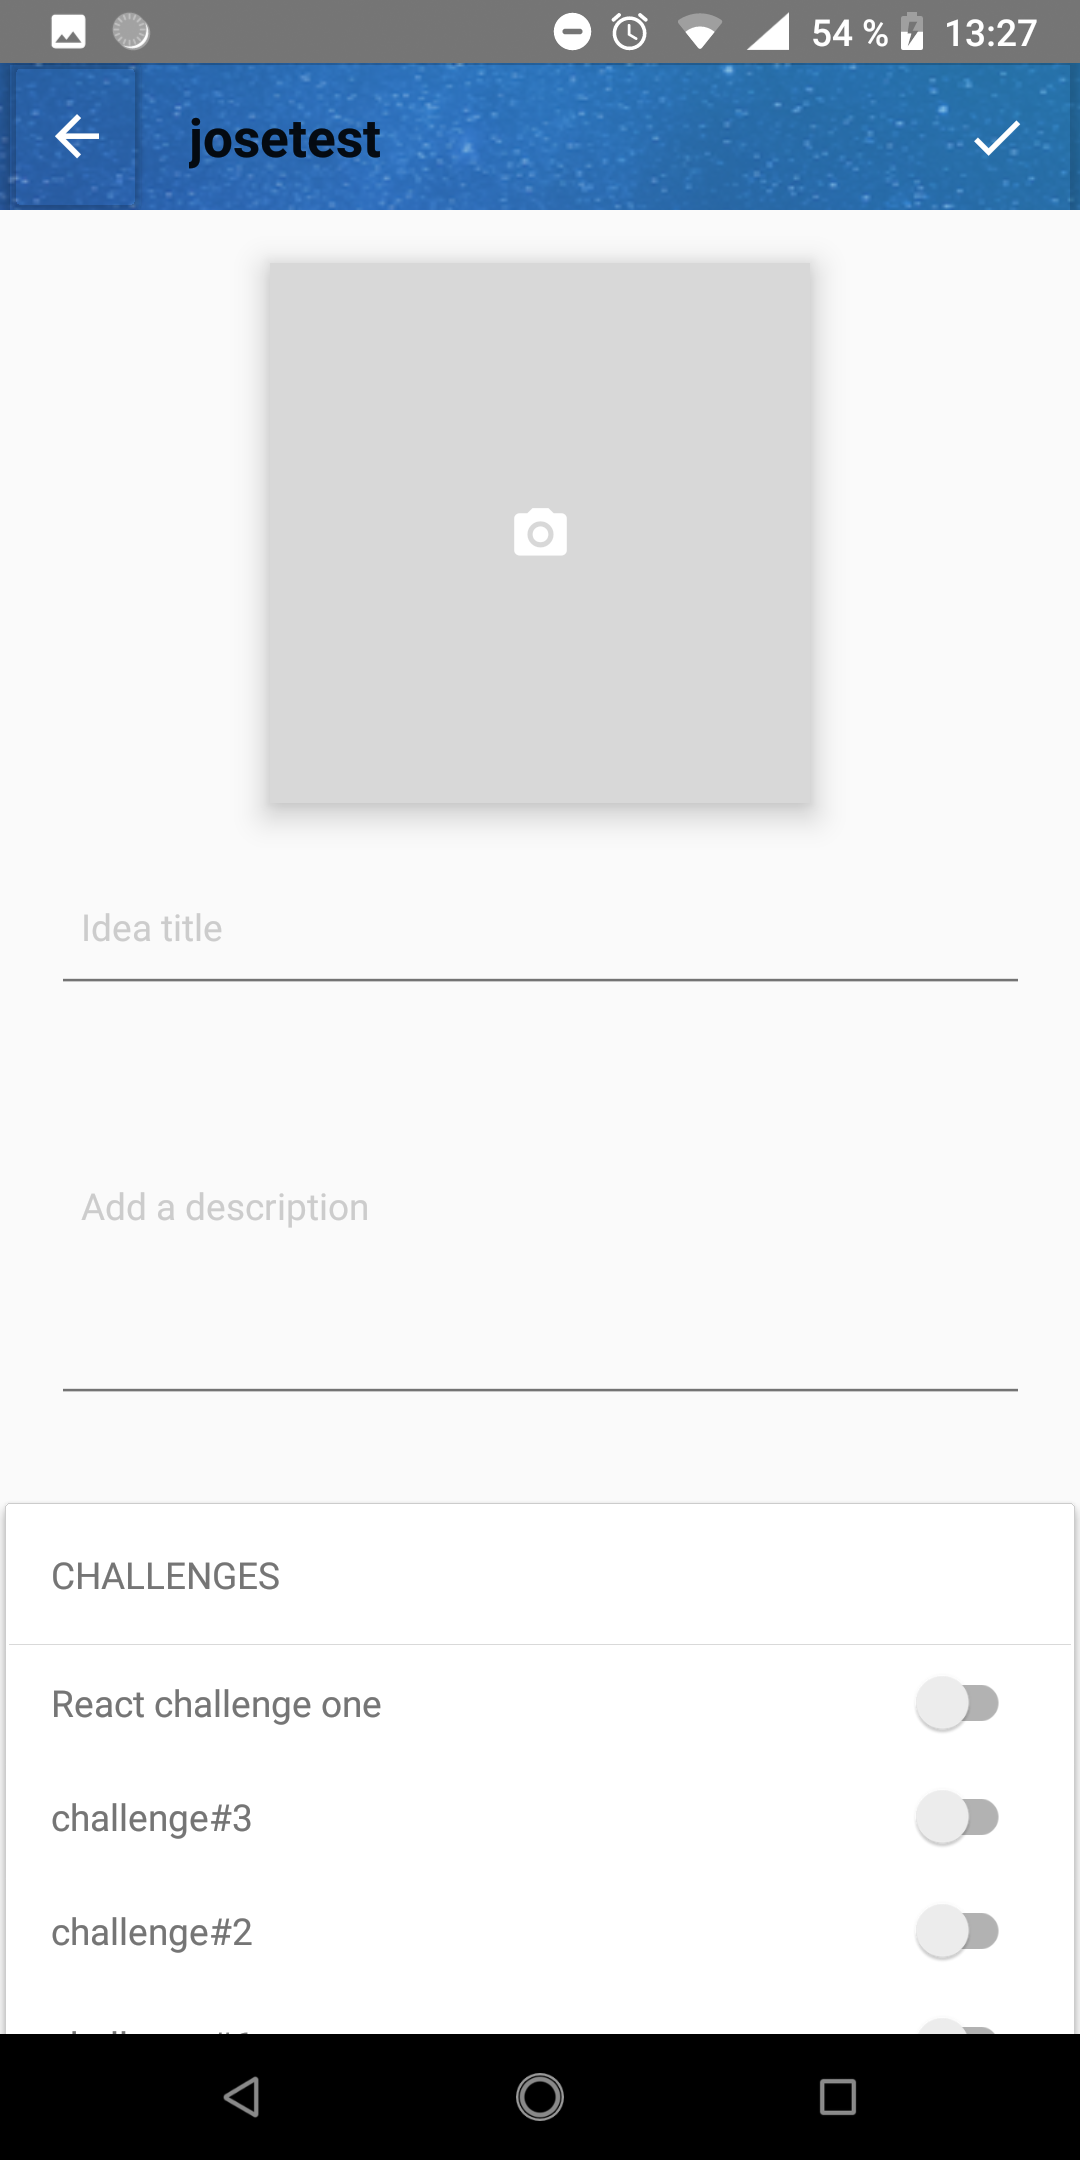
\includegraphics[width=0.3\textwidth]{./img/anexo1/crear_idea.png}
		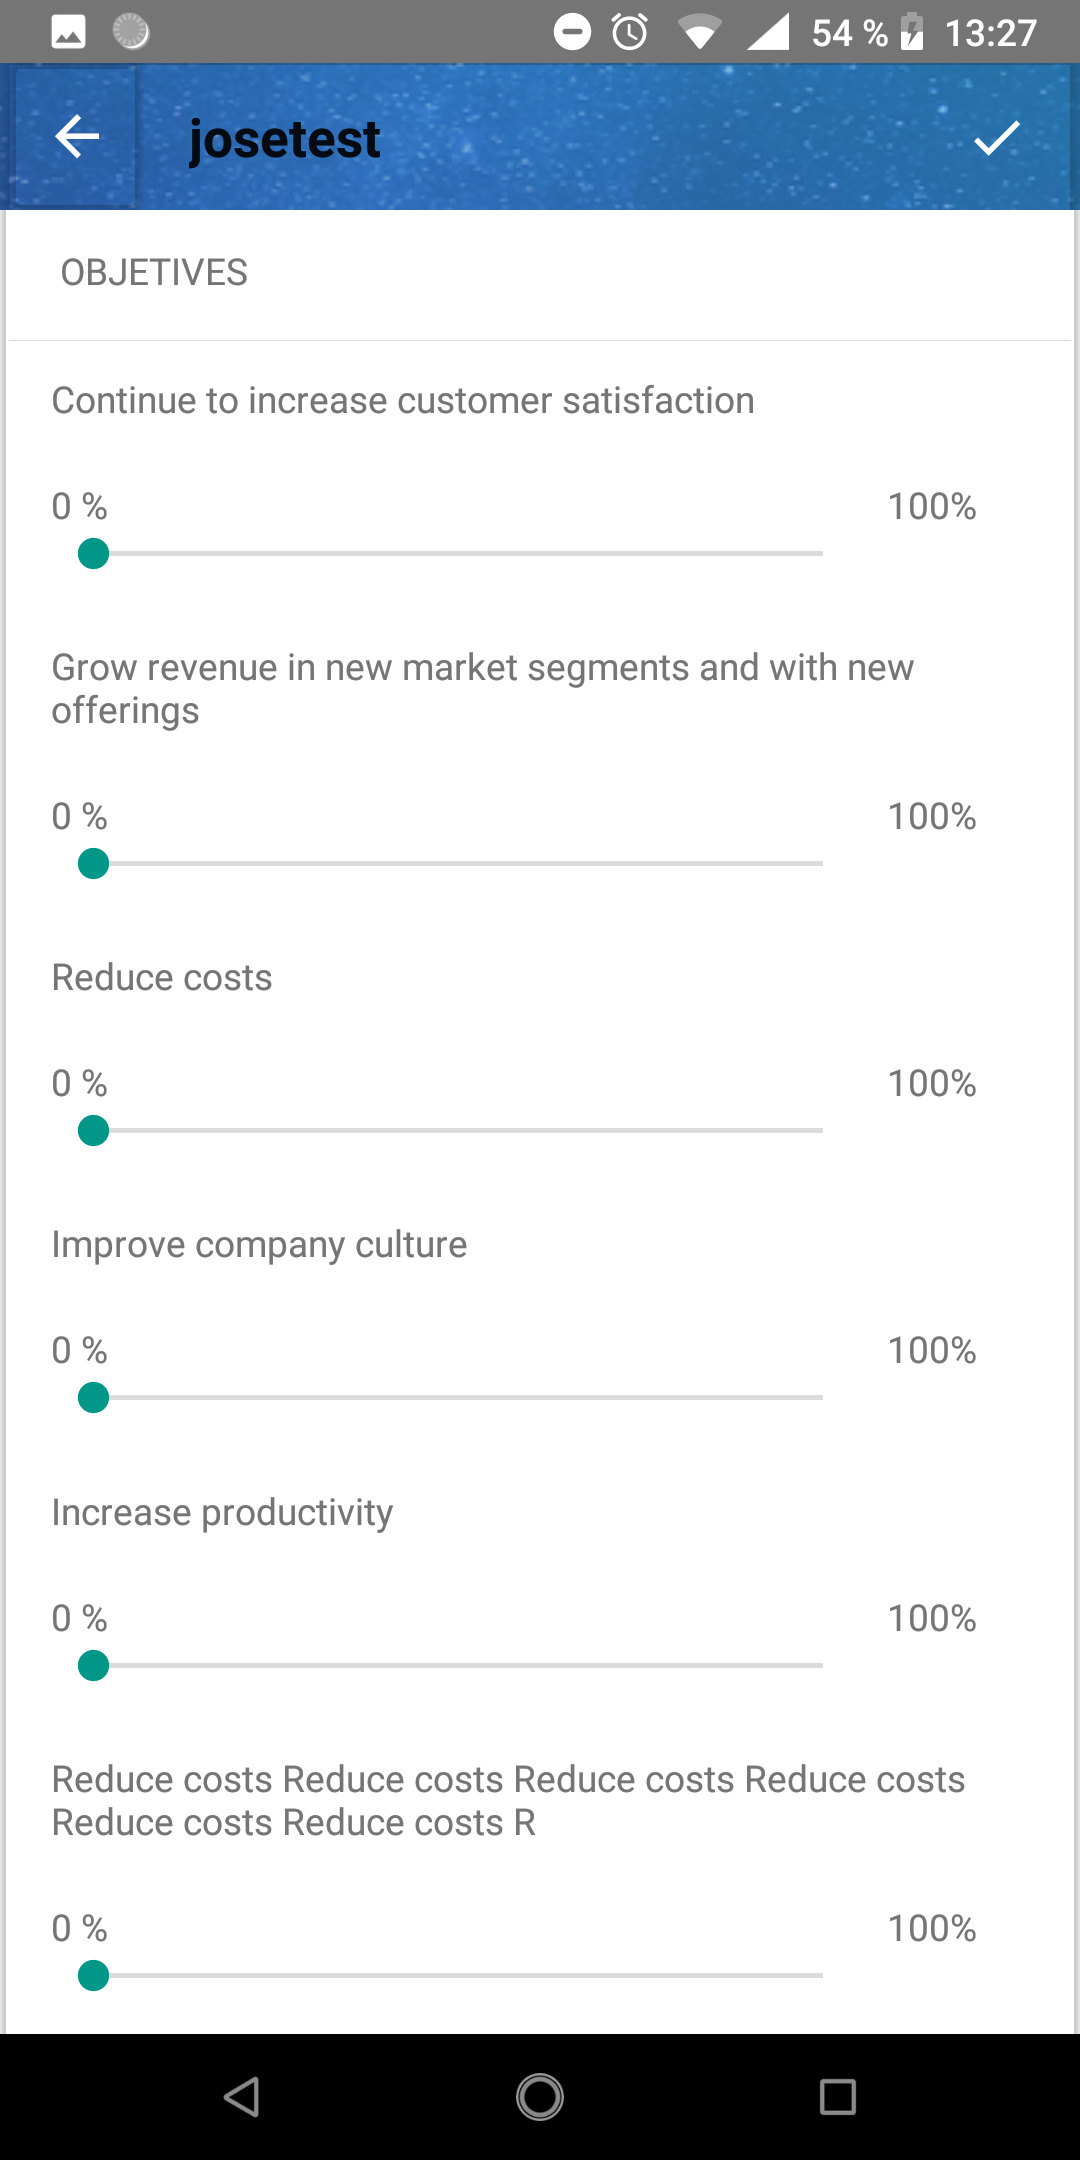
\includegraphics[width=0.3\textwidth]{./img/anexo1/crear_idea_cont.png}
		\caption{Formulario de crear idea}
		\label{fig:crear_idea}
	\end{center}
\end{figure}

\section{Desafíos}

Una vez que se entra a un desafío, se ve una pestaña que muestra la información más 
relevante del desafío (ver figura~\ref{fig:ver_desafio_inicio}), como el titulo, el autor, el 
patrocinador, los días restantes o una descripción. 

\begin{figure}[!h]
	\begin{center}
		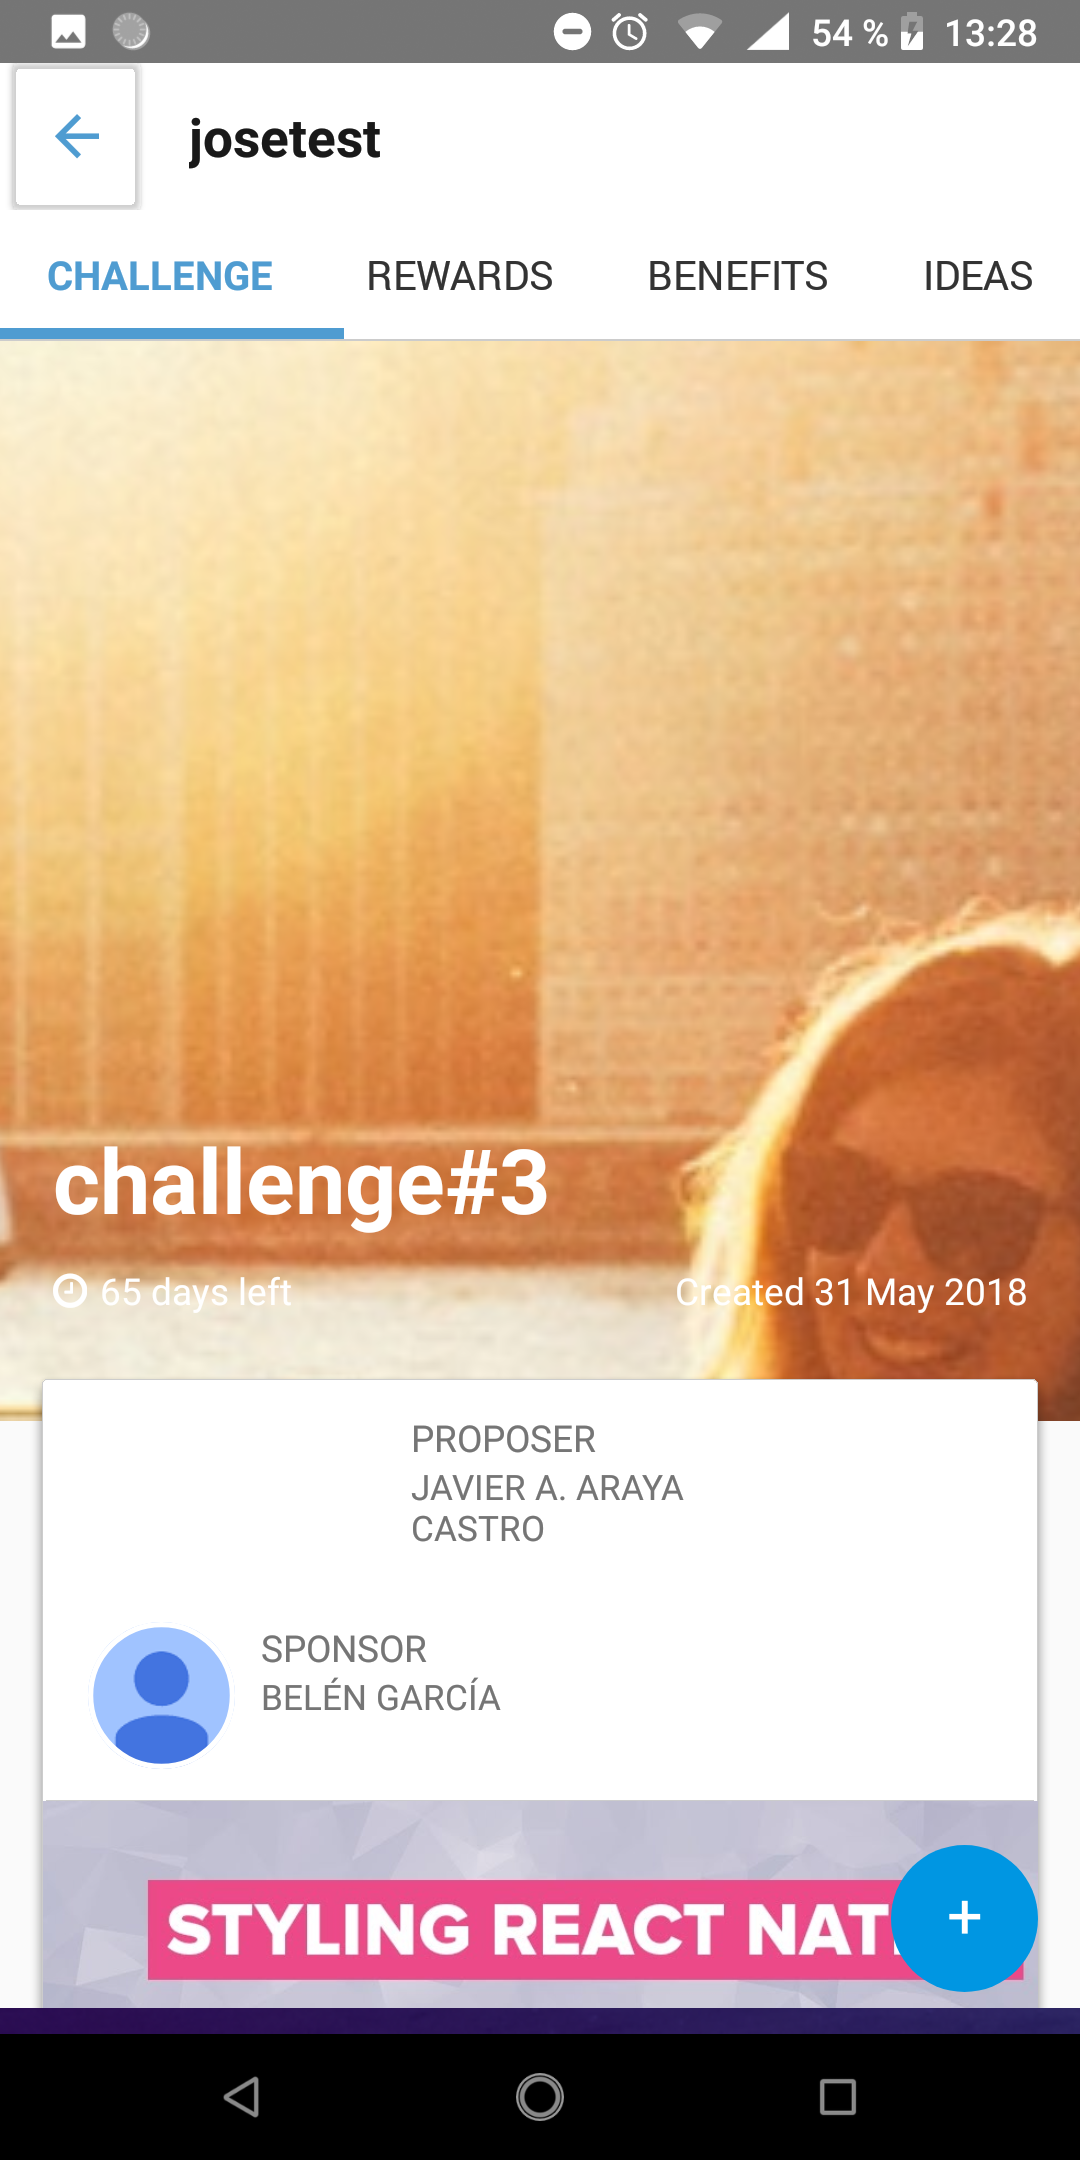
\includegraphics[width=0.3\textwidth]{./img/anexo1/ver_desafio_inicio.png}
		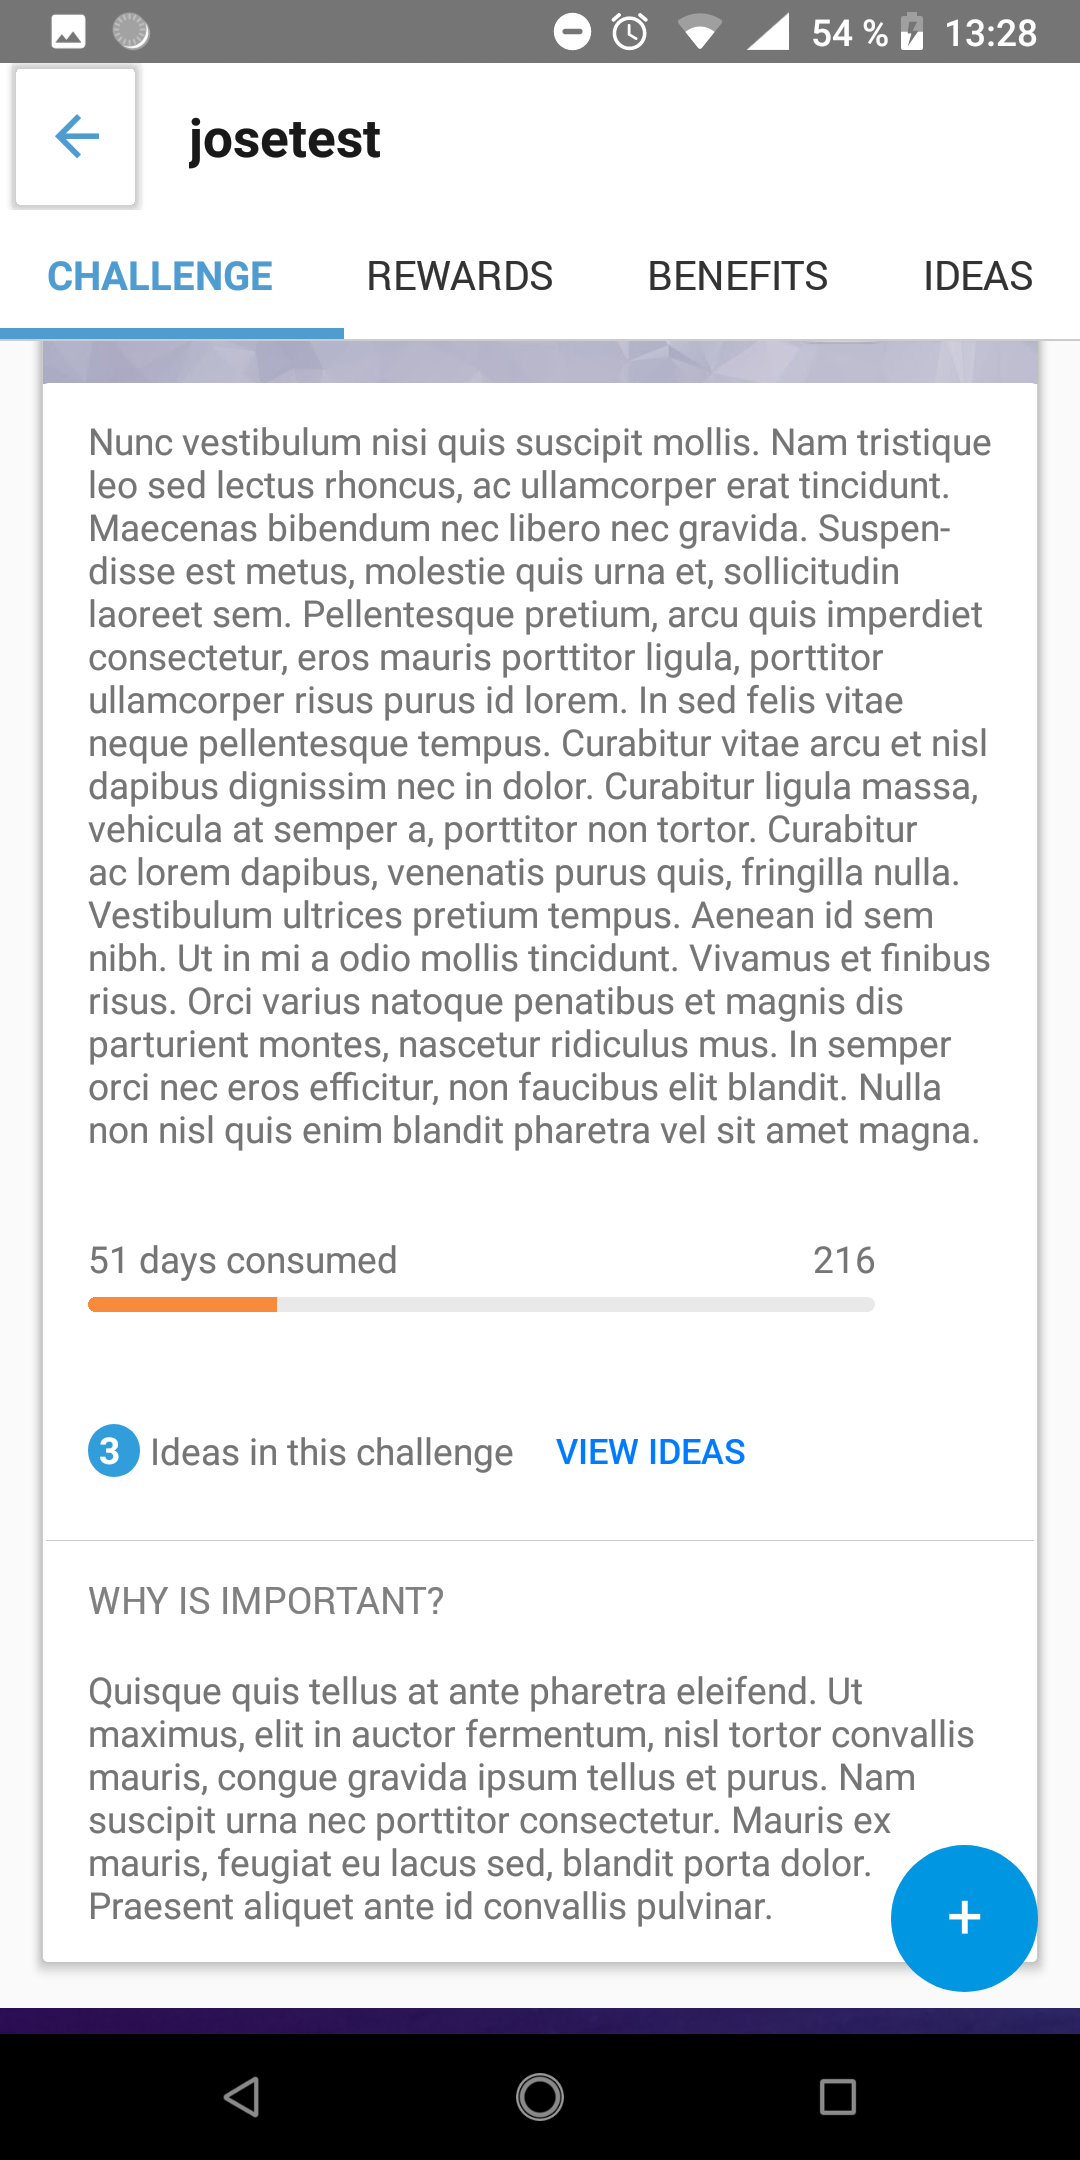
\includegraphics[width=0.3\textwidth]{./img/anexo1/ver_desafio_inicio_cont.png}
		\caption{Pantalla inicial de la información del desafío}
		\label{fig:ver_desafio_inicio}
	\end{center}
\end{figure}

En la pestaña de ideas o pulsando en «Ver ideas» de la pestaña principal se accede a la 
pantalla que lista las ideas pertenecientes al desafío (ver figura~\ref{fig:ver_desafio_ideas}).

\begin{figure}[!h]
	\begin{center}
		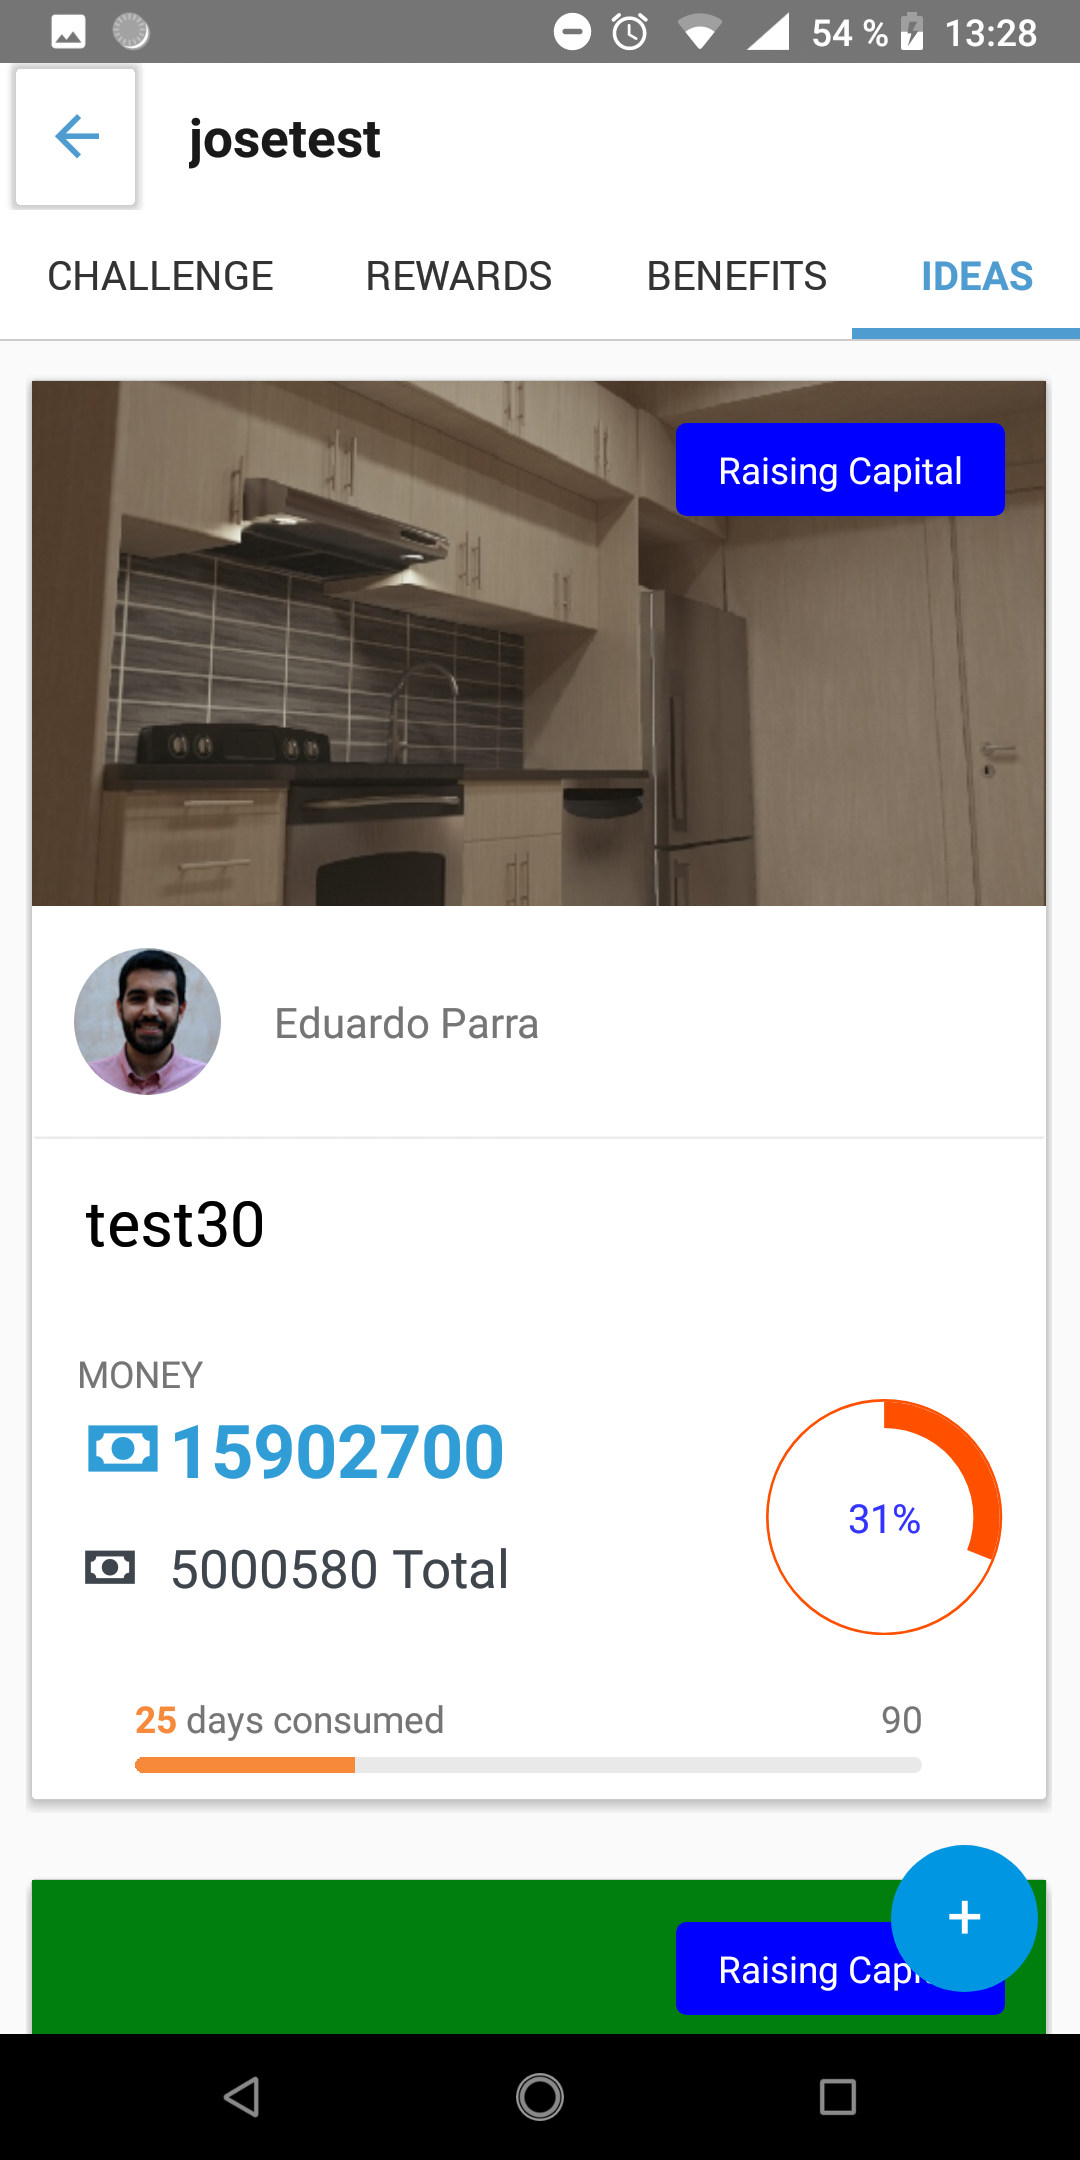
\includegraphics[width=0.3\textwidth]{./img/anexo1/ver_desafio_ideas.png}
		\caption{Pantalla con las ideas pertenecientes al desafío}
		\label{fig:ver_desafio_ideas}
	\end{center}
\end{figure}

En la pestaña de beneficios (ver figura~\ref{fig:ver_desafio_beneficios}), si la tiene el desafío, 
se muestran los multiplicadores de dinero en el caso de que alguna de las ideas de ese 
desafío sea aprobada, soportada o implementada.

\begin{figure}[!h]
	\begin{center}
		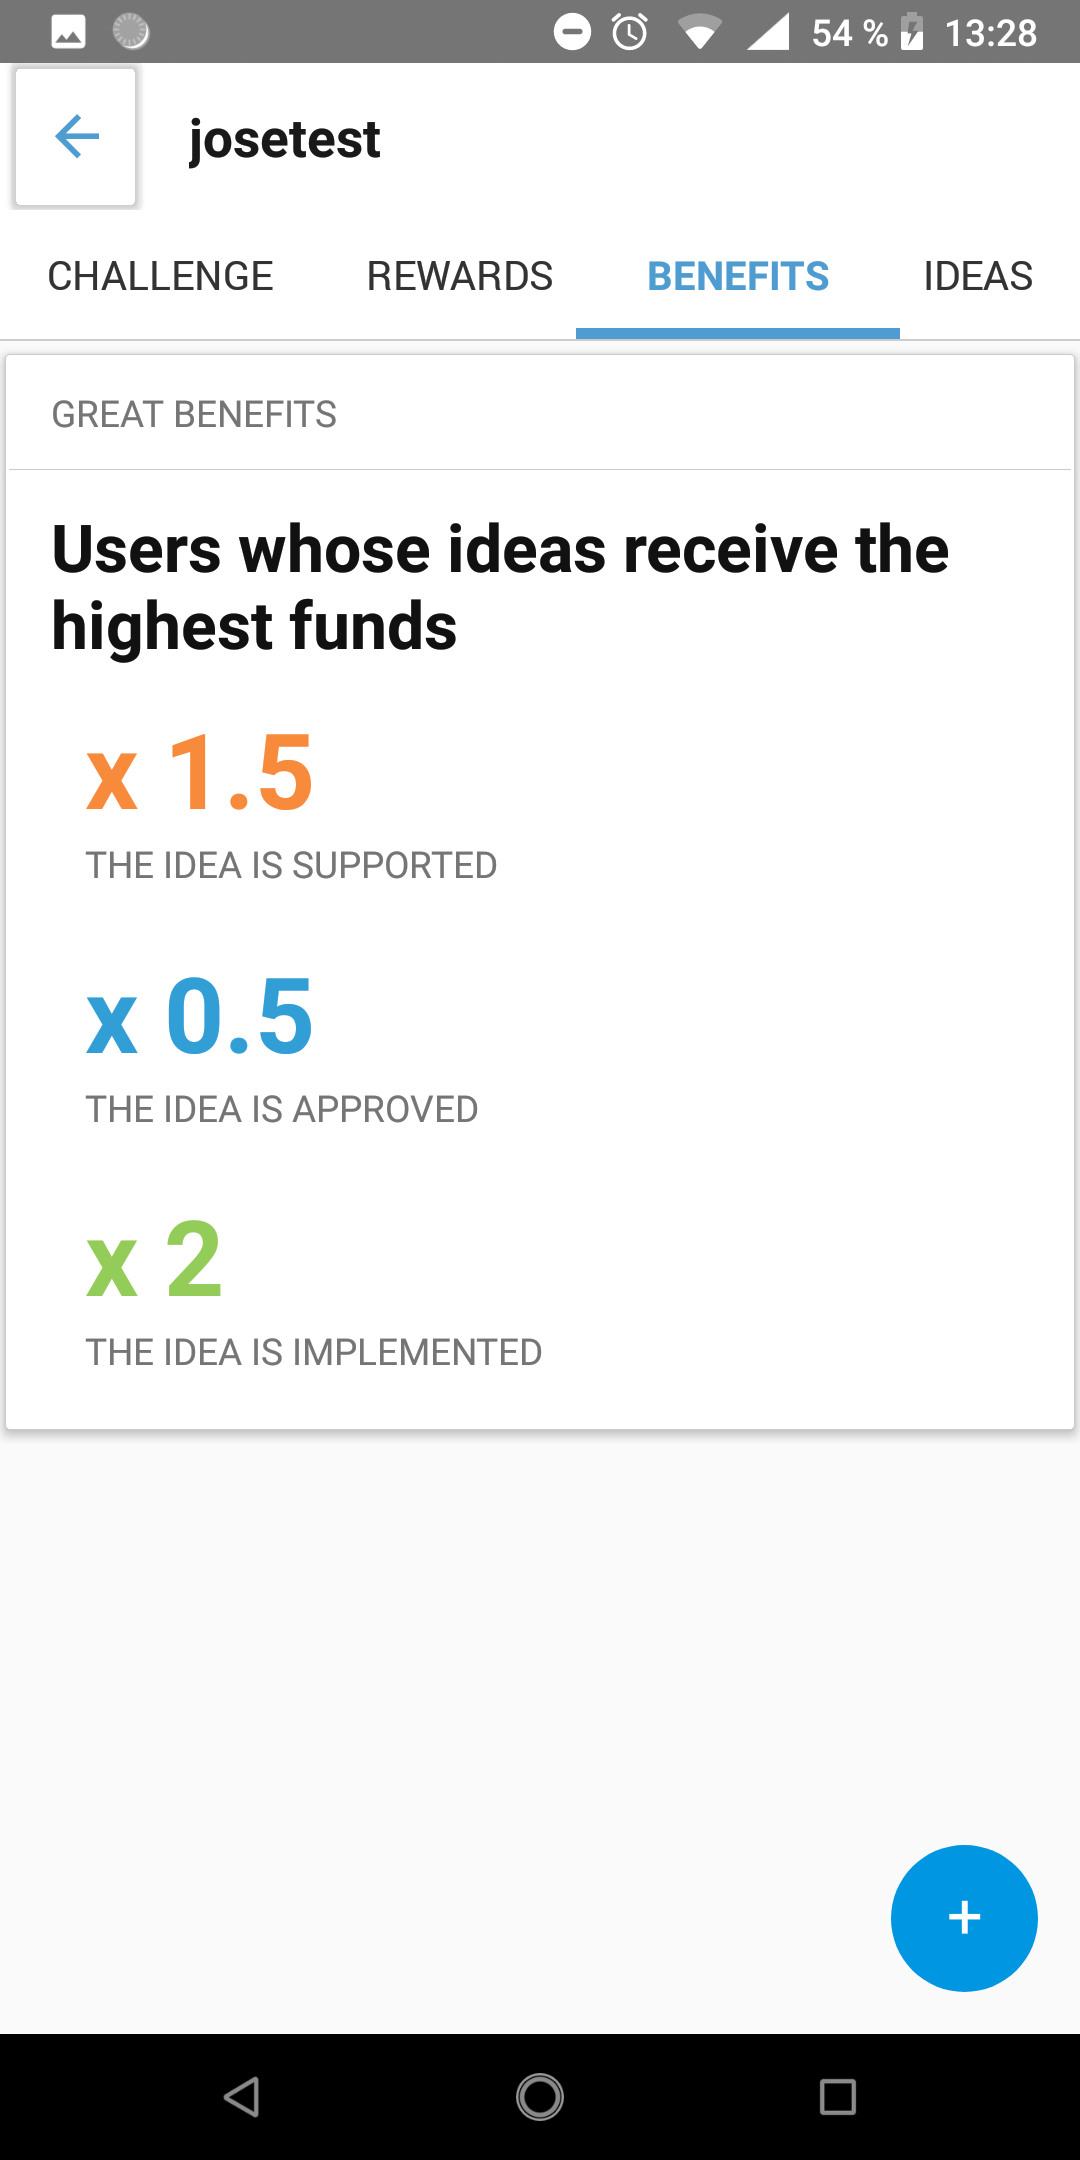
\includegraphics[width=0.3\textwidth]{./img/anexo1/ver_desafio_beneficios.png}
		\caption{Pantalla de beneficios del desafío}
		\label{fig:ver_desafio_beneficios}
	\end{center}
\end{figure}


\section{Notificaciones}

Se puede acceder a la pantalla de notificaciones desde el menú lateral, hay tres pestañas 
(ver figura~\ref{fig:notificaciones}) en la primera se muestran las notificaciones del usuario 
y la actividad del Nextinit y en las otras dos se muestra las notificaciones y la actividad 
por separado.

\begin{figure}[!h]
	\begin{center}
		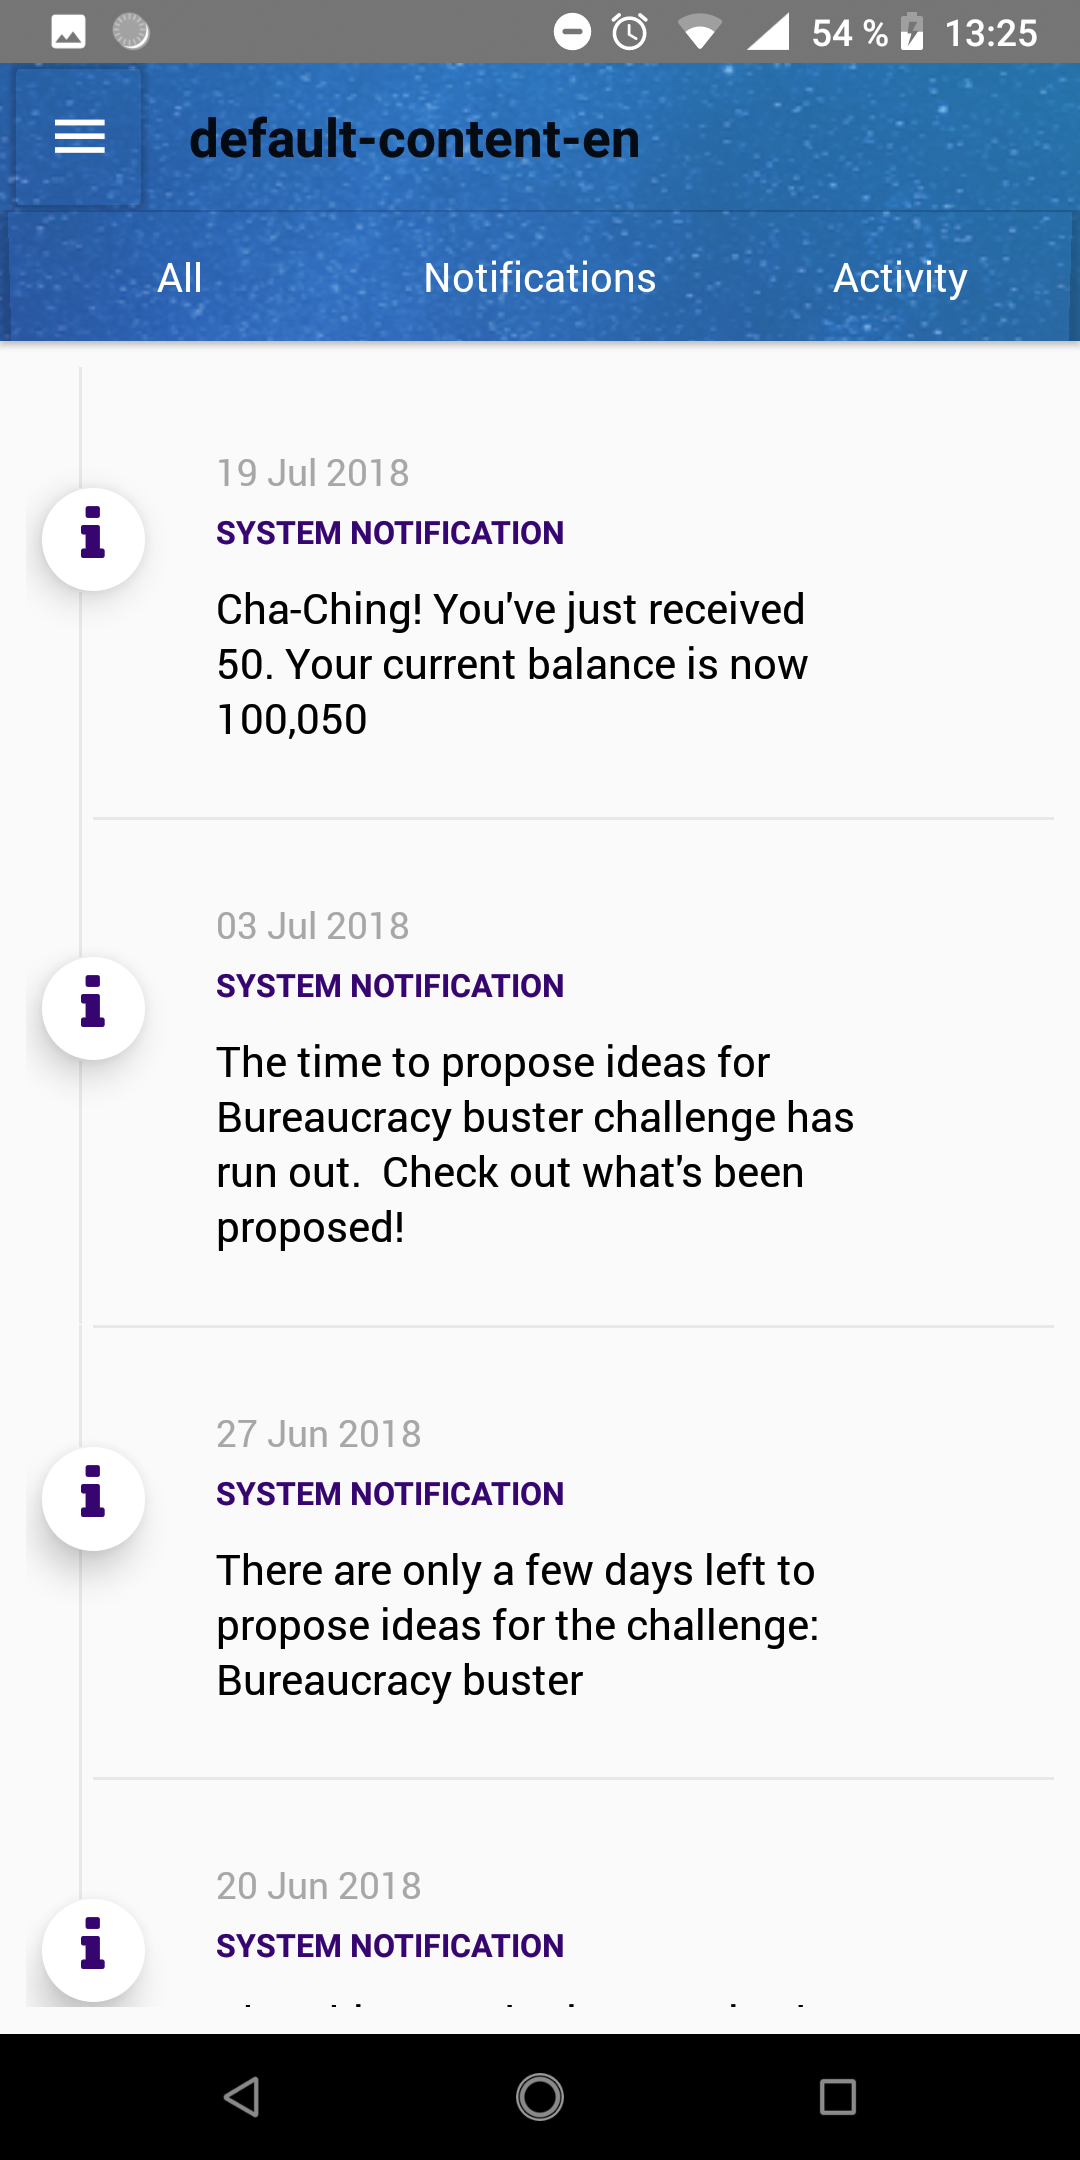
\includegraphics[width=0.3\textwidth]{./img/anexo1/notificaciones_all.png}
		\caption{Pantalla de notificaciones}
		\label{fig:notificaciones}
	\end{center}
\end{figure}

\section{FAQ}
